\documentclass{article}
\usepackage{subfig}
\usepackage{multirow}
\usepackage{tabularx}
\usepackage{placeins}
\usepackage{subfig}
\usepackage{graphicx}
\usepackage{caption}
\usepackage{float}
\usepackage{hyperref}
\usepackage{array}
% if you need to pass options to natbib, use, e.g.:
%     \PassOptionsToPackage{numbers, compress}{natbib}
% before loading neurips_2020

% ready for submission
% \usepackage{neurips_2020}

% to compile a preprint version, e.g., for submission to arXiv, add add the
% [preprint] option:
    % \usepackage[preprint]{neurips_2020}

% to compile a camera-ready version, add the [final] option, e.g.:
    \usepackage[final]{neurips_2020}

% to avoid loading the natbib package, add option nonatbib:
    %  \usepackage[nonatbib]{neurips_2020}
\usepackage{listings}
\usepackage[utf8]{inputenc} % allow utf-8 input
\usepackage[T1]{fontenc}    % use 8-bit T1 fonts
\usepackage{hyperref}       % hyperlinks
\usepackage{url}            % simple URL typesetting
\usepackage{booktabs}       % professional-quality tables
\usepackage{amsfonts}       % blackboard math symbols
\usepackage{nicefrac}       % compact symbols for 1/2, etc.
\usepackage{microtype}      % microtypography
\usepackage{xcolor}
\usepackage{placeins}       % in-place positioning of figures/tables
\usepackage{graphicx}
\usepackage{adjustbox}
\renewcommand{\arraystretch}{1.5}
\definecolor{codegreen}{rgb}{0,0.6,0}
\definecolor{codegray}{rgb}{0.5,0.5,0.5}
\definecolor{codepurple}{rgb}{0.58,0,0.82}
\definecolor{backcolour}{rgb}{0.95,0.95,0.92}

\lstdefinestyle{mystyle}{
    backgroundcolor=\color{backcolour},   
    commentstyle=\color{codegreen},
    keywordstyle=\color{magenta},
    numberstyle=\tiny\color{codegray},
    stringstyle=\color{codepurple},
    basicstyle=\ttfamily\footnotesize,
    breakatwhitespace=false,         
    breaklines=true,                 
    captionpos=b,                    
    keepspaces=true,                 
    numbers=left,                    
    numbersep=5pt,                  
    showspaces=false,                
    showstringspaces=false,
    showtabs=false,                  
    tabsize=2
}

\lstset{style=mystyle}
\title{Youtube Educational Content Analysis\\\\
\large{Group 17}}

% The \author macro works with any number of authors. There are two commands
% used to separate the names and addresses of multiple authors: \And and \AND.
%
% Using \And between authors leaves it to LaTeX to determine where to break the
% lines. Using \AND forces a line break at that point. So, if LaTeX puts 3 of 4
% authors names on the first line, and the last on the second line, try using
% \AND instead of \And before the third author name.
\author{%
  Ayush Kumar\\
%   Indian Institute of Technology\\
%   Kanpur \\
Roll No: 170195\\
  \texttt{ayushk@iitk.ac.in} \\
  % examples of more authors
   \And
   Harsh Agarwal \\
   %   Indian Institute of Technology\\
%   Kanpur \\
Roll No: 170287\\
   \texttt{harshaga@iitk.ac.in} \\
   \AND
   Keshav Bansal\\
   %   Indian Institute of Technology\\
%   Kanpur \\
Roll No: 170335\\
  \texttt{keshavb@iitk.ac.in} \\
   \And
   Snehal Raj\\
   %   Indian Institute of Technology\\
%   Kanpur \\
Roll No: 170705\\
  \texttt{snehal@iitk.ac.in} \\
   \And
  Umang Malik\\
   %   Indian Institute of Technology\\
%   Kanpur \\
Roll No: 170765\\
  \texttt{umangmal@iitk.ac.in} \\
}
\begin{document}
\maketitle

\begin{abstract}
YouTube has served as a free education sharing platform for over a decade now. Various colleges around the world have set up multiple organizations to put out some content for free. Even independent creators have also gained a large audience on YouTube. Through this project, we analyze the educational domain videos to draw insights that can improve the quality of content currently being delivered by content creators and instructors on the platform.
\end{abstract}
\section{Problem Statement}
Educational videos can enhance learning and easily integrate into standard instructional methods. Studies have shown that the use of short video clips allows for more efficient processing and memory recall. The visual and auditory nature of videos appeals to a broad audience and allows each user to process information in a way that’s natural to them. YouTube permits worldwide access to high-quality educational videos; however, not many studies have described the reach of educational videos on YouTube or what topics are preferred. 

The aim of this project is to contribute towards a better understanding of the content that is being shared in the educational videos published on the YouTube. The main goals of this project are as follows :
\begin{itemize}
    
\item Providing a comprehensive dataset of the educational video statistics  on Youtube including college and branch specific content of NPTEL.
\item Analysing what factors affecting the popularity of an educational video on Youtube by studying the correlation between various evaluation metrics.
\item Analysis of  educational content in India vs other countries based on topics covered, video length, views-like ratio.
    \item Using the playlist of topics to identify peaks and troughs and suggesting topics which needs improvement in future iterations.
    
\end{itemize}

\section{Introduction and Motivation}
The evolution of the web and the emergence of online mode of education has enabled new levels of interaction and communication for learning. This also has led to an increase in the responsibilities of teachers, students and educational institutions.
Universities are now facing the need to adapt and enter into the online space, evolving into a University 2.0 . Taking advantage of students strong interactions in those online environments, as YouTube or Facebook, universities are trying to move closer to them, establishing their official presence in the same online places. Despite this, many higher education institutions are cautious of the extent that their presence should have in these web platforms.

Through this project, we aim to analyse the educational content put forth by top creators in India and worldwide. The content examined includes videos from topmost universities like IITs (NPTEL) and MIT (MIT Open Courseware) and independent creators like Khan academy and Unacademy. 

This project will help us to identify ways in which these content creators can increase the reachability and likeness of their content, thereby making education more accessible to the masses as well as making it a profitable venture for the creator.

Further, we aim to analyse trends which help us distinguish the educational demand in India from other countries, thereby assisting creators in knowing the requirements of Indian students.

Since lots of colleges have shifted to the online mode of delivery due to COVID, analysis of existing educational videos becomes even more critical. This analysis will also help in the upcoming semesters, which are expected to be online as well.
\section{Datasets Required}
For this project, we used the YouTube Data API for obtaining several statistics for some of the most popular educational content distributors on YouTube. The various aspects and limitations of the API are described in the latter section. First, we describe a list of channels that we focus our analysis on and then we describe the data collected for each of them.\\
% \newpage
\subsection{Channels}
\begin{enumerate}
    \item \textbf{NPTEL}: NPTEL, founded by the Indian Institutes of Technology and the Indian Institute of Science, serves as the primary channel for hosting recorded lectures and tutorials from these premier institutes for undergraduate and masters students. The channel covers all introductory engineering courses along with other humanities and life sciences courses as well.\\
    \item \textbf{MIT OpenCourseWare}: Managed by the Massachusetts Institute of Technology, this channel publishes study material from its undergraduate and graduate-level courses. It is the American counterpart of NPTEL.\\
    \item \textbf{Khan Academy}: This channel offers free online courses for Intermediate and High School students. Unlike the others, it does not cater to the undergraduate or graduate audience.\\
    \iffalse
    \item \textbf{Coursera}: Coursera, started by Stanford professors, is well renowned as the hotspot of all online learning. It contains a mix of high school, undergraduate and graduate-level courses. Other than this, it also offers specializations, degrees, professional and master track courses on several topics assembled from different institutes worldwide.\\
    \item \textbf{Udemy}: Udemy is another American MOOC (Massive Open Online Course) provider similar to Coursera.\\
    \fi
    \item \textbf{Unacademy JEE}: Unacademy is another Indian channel targeting high school students preparing for several entrance examinations in Engineering, Medical and other streams.\\
    \item \textbf{Study IQ Education}: This is another Indian channel providing short online classes covering general topics for students preparing for the UPSC entrance examinations.\\
    \item \textbf{Physics Wallah}: This is an Indian channel started by Alakh Pandey which provides free online Physics courses meant explicitly for High School students in India preparing for the Joint Entrance Examinations.\\
\end{enumerate}
A figurative analysis of the number of playlists and the number of videos uploaded by each channel is provided below in figure \ref{fig:channel_info} \footnote{Data obtained as of November, 2020}.
\begin{figure}[!htp]
    \centering
    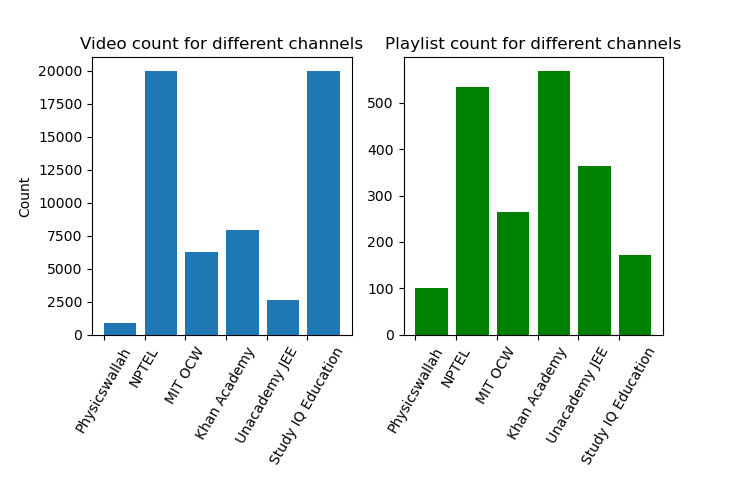
\includegraphics[scale = 0.50]{images/videos_playlist_count.png}
    \caption{Comparison of number of videos and playlists uploaded by different channels}
    \label{fig:channel_info}
\end{figure}
\Floatbarrier

\newpage
\section{Data Retrieval: Youtube Data API}
For each of the channels stated above, we collect data for all videos of the channel on youtube. This includes : 
\begin{itemize}
    \item Title
    \item Likes/Dislikes
    \item Comments
    \item Views
    \item Video Description
    \item Tags
    \item Upload date
    \item Video Length
\end{itemize}
Below is a short description on APIs used to populate the data.
\begin{enumerate}
    \item \textbf{Channels API\footnote{\url{https://developers.google.com/youtube/v3/docs/channels}}:} We use this API to find all `uploads' of the channel.
    \item \textbf{Playlists API\footnote{\url{https://developers.google.com/youtube/v3/docs/playlists}}:} Using this API we can get ids of all the playlists which are part of a particular channel. These playlists mostly represent course playlists in NPTEL/MIT OCW.
    \item \textbf{PlaylistItems API\footnote{\url{https://developers.google.com/youtube/v3/docs/playlistItems}}:} Using this API, we get \textit{videoId} for all videos which are part of the playlist.
    \item \textbf{Videos API\footnote{\url{https://developers.google.com/youtube/v3/docs/videos}}:} After we have \textit{videoId}'s for all the videos (uploads by channel or part of playlist). We get the data for each video which includes Title, Likes, Views, etc. This API does not provide comments.
    \item \textbf{CommentThreads API\footnote{\url{https://developers.google.com/youtube/v3/docs/commentThreads}}:} Using this API we get Comments for a particular video on youtube. 
\end{enumerate}

\subsection{Data Indexing}
The data after extraction is stored (or indexed) in multiple JSON files. We use these JSON files to apply mining techniques to obtain useful insights from the extracted data. This section explains the structure of the JSON files.
\begin{itemize}
    \item \texttt{video\_ids.json}: This file contains video IDs of all videos present inside the above listed six YouTube channels. 
    \item \texttt{all\_playlist.json}: This file contains playlists and videos ids for videos which are part of that playlist for each channel.
    \item \texttt{all\_videos.json}: This file contains map of video IDs and data for the corresponding video. Data includes: Title, Likes/ Dislikes count, Views, Video Description, Title, etc. Note that this data does not contain comments. 
    \item \texttt{comments.json}: This file contains the comments text and likes on that comment, for all videos. We have ignored videos where comment count was less than 5 and we have only scrapped maximum of 50 comments per video. 
\end{itemize}
Aside from the above files which we have scraped using the YouTube Data API, we have some processed files in the /data folder (For example, after applying sentiment analysis, clustering etc.) 

% **               likeCount  viewCount  commentCount
% likeCount      1.000000   0.810523      0.935411
% viewCount      0.810523   1.000000      0.783737
% commentCount   0.935411   0.783737      1.000000
% ** physics_wallah               likeCount  viewCount  commentCount
% likeCount      1.000000   0.927984      0.896052
% viewCount      0.927984   1.000000      0.783352
% commentCount   0.896052   0.783352      1.000000
% ** nptel               likeCount  viewCount  commentCount
% likeCount      1.000000   0.902254      0.812515
% viewCount      0.902254   1.000000      0.779864
% commentCount   0.812515   0.779864      1.000000
% ** mit               likeCount  viewCount  commentCount
% likeCount      1.000000   0.912579      0.851227
% viewCount      0.912579   1.000000      0.817555
% commentCount   0.851227   0.817555      1.000000
% ** khan_academy               likeCount  viewCount  commentCount
% likeCount      1.000000   0.737639      0.891568
% viewCount      0.737639   1.000000      0.683877
% commentCount   0.891568   0.683877      1.000000
% ** unacademy_jee               likeCount  viewCount  commentCount
% likeCount      1.000000   0.947753      0.914989
% viewCount      0.947753   1.000000      0.852628
% commentCount   0.914989   0.852628      1.000000
% ** study_iq_education               likeCount  viewCount  commentCount
% likeCount      1.000000   0.947228      0.825841
% viewCount      0.947228   1.000000      0.843698
% commentCount   0.825841   0.843698      1.000000


% (IITK, CSE, 528, 7114.051, 26.159, 0.948)
% (IITD, CSE, 503, 44451.089, 107.056, 0.943)
% (IITB, CSE, 188, 58259.101, 132.601, 0.939)
% (IITM, CSE, 530, 42674.226, 123.460, 0.938)
% (IITKGP, CSE, 764, 38803.469, 92.077, 0.937)

% (IITM, ME, 845, 11474.535, 55.231, 0.964)
% (IITK, ME, 804, 23718.689, 76.672, 0.962)
% (IITB, ME, 403, 30586.285, 95.814, 0.960)
% (IITKGP, ME, 1059, 31227.553, 119.791, 0.957)
% (IITD, ME, 228, 32261.667, 113.474, 0.940)

% (IITK, EE, 554, 20808.715, 65.722, 0.960)
% (IITD, EE, 664, 52339.633, 129.443, 0.953)
% (IITM, EE, 1088, 41959.692, 134.225, 0.953)
% (IITB, EE, 904, 25270.758, 67.833, 0.944)
% (IITKGP, EE, 935, 35999.903, 97.142, 0.937)

% (IITB, CHE, 155, 4378.987, 24.690, 0.963)
% (IITK, CHE, 121, 10061.661, 38.372, 0.962)
% (IITM, CHE, 392, 6379.497, 34.115, 0.960)
% (IITKGP, CHE, 280, 6292.718, 22.954, 0.959)
% (IITD, CHE, 40, 1345.050, 5.025, 0.905)

% \section{Methodology and Analysis}
% From the data populated using youtube API. We employ various data mining methods on this data to get interesting insights.

% \begin{itemize}
%     \item \textbf{Video Description}:
%     \begin{enumerate}
%         \item Using named entity recognition algorithms, we aim to extract fields like college name, department and course topics which will be further useful for aggregating and comparing results for each department/subject.
%         \item We can rank each topic of college based on the aggregated number of views/likes.

%     \end{enumerate}
%     \item \textbf{Comments}:
%     \begin{enumerate}
%         \item We propose to use a sentiment analysis model to classify each comment as positive, neutral or negative. Based on this, we can calculate a total polarity score of all the comments. Using this, we plan to use correlation analysis to study the relation of the polarity of comments with other properties such as likes, views, topic etc.
%         \item For NPTEL, we expect a significant proportion of comments to be in mixed language (such as Hindi-English). To ensure proper analysis of such comments, we will use a multilingual model for embeddings, which have been proven to work well on such texts \cite{qin2020cosdaml}.
%     \end{enumerate}
%     \item \textbf{Correlation Analysis}:
%     \begin{enumerate}
%         \item We plan to use correlation analysis to find the relationship between variables. For example, the trend of the polarity of comments with views/likes, number of views with likes, etc.
%         \item For this, we will use Chi-square test \cite{chisquare} or Pearson correlation. 
%     \end{enumerate}
%     \item \textbf{Identifying Playlist (or course) peaks and troughs}:
%     \begin{enumerate}
%         \item We can decide the peaks and troughs in playlists by seeing which videos have maximum and minimum z-score (i.e. deviating most from the mean) according to the distribution of views/likes. 
%         \item We will rank the videos in a playlist according to z-score and will identify whether a topic appears as a peak in one channel and trough in another.
%     \end{enumerate}
% \end{itemize}








% \section{Expected Outcomes}

% At the conclusion of the project, we aim to achieve the following results pertaining to our analyses performed on the different educational channels listed above:

% \begin{itemize}
%     \item \textbf{Popularity of Courses}: We want to be able to benchmark and compare the popularity of different course topics across different channels. This will enable us to draw parallels between the course contents of similar courses on different channels and their corresponding responses from the audience in terms of views, comments and likes.
%     \item  \textbf{Insights about colleges}: Insights about the topics taught at different colleges such as \textit{``IIT Kanpur has highly positive reviews for Mathematics related courses"}, \textit{``IIT Bombay offers lots of courses from its Electrical Engineering department"}
%     \item \textbf{Hotspot topics in a course (playlist)}: Analyzing the playlist of individual courses, we will find the topics which are popular in that particular course. 
    
%     \item \textbf{Relation between metadata}: From our analysis, we expect that we will observe a positive correlation between variables. For example, the trend of the polarity of comments with views/likes, number of views with likes, etc.
    
%     \item \textbf{Optimal Video Length}: From our analysis, we aim to determine the ideal length of a lecture/tutorial video that garners the best response from the students. It has been proposed that shorter educational videos are preferred. This fact needs to be verified.
    
%     \item \textbf{Suggestions about course offering:} By comparing the video ratings for topics on NPTEL and foreign channels, we will suggest which courses should be offered by NPTEL in the future.
% \end{itemize}
\section{Methodology}
\subsection{Video Length}
We carried out an analysis on the variation  of parameters such as number of views, number of likes and number of comments with the length of video (in seconds). This analysis will be useful for educational content creators to decide the optimal length of their videos such that it gains maximum reach and/or is monetarily profitable.   

To understand this variation with the length of video, we plotted bar-plots and box-plots with the number of likes/views/comments on the Y-axis and length of video in X-axis. For this we used the data contained in the file  \texttt{all\_videos.json}, which contains all these parameters for each of the videos used by us.

The results for this are shown in section \ref{video_length}



\subsection{Correlation between Frequency of Likes, Views and Comments}
The number of views, likes or comments gathered by a YouTube video is indicative of a video's reachability and its likeness to the public. It is important to understand the correlation between these attributes for understanding the YouTube algorithm better. Its also not straightforward to identify the trend, since we see quite often that videos that are highly viewed might also contain a lot of dislikes.  

We use the Spearman rank correlation method for finding the pairwise degree of association between the three variables. The results for this are described at Section \ref{correlation}.

\subsection{College Ranking Analysis}
% To perform college specific analysis. Including relative comparison of quality of videos uploaded by each college. And performing branch-wise comparison between different colleges. To perform this analysis I use videos uploaded on nptel's youtube channel. 

We also tried performing college-specific analysis by comparing the videos uploaded by each college to NPTELHRD's channel. 
However, the videos on the channel aren't separated by universities directly. So, we used the metadata from each youtube video on the channel, and separated them college wise. We  built a named entity recognition (NER) model to give college tags to the videos. This NER model uses parts of speech (POS) tagging, which helps us identify nouns in the video description then we perform similarity matching on these nouns with college names. 

We used this similarity matching to account for videos uploaded with a spelling mistake in the name of the college. This method took care of those spelling mistake, and other noises present due to human error. The extracted videos for each college are further tagged with branch names. We again use the same NER model, but this time we are performing similarity matching with branch names. 

After video filtering several analysis were performed on the metadata from these videos. The results and discussion for this are shown in section \ref{collge_rank}

\subsection{Playlist Retention}
To find how the views decline as a course (playlist) progresses, we start from the 3rd video of the course. This is because the first two courses have lots of non-serious views. We then find the percentage of views (compared to the third video) as the course progresses. This signifies the retention of students in a course.

Then, we find the median of these percentages at each position in a playlist to get the general trend of playlist progression. This exercise was done for multiple channels to get an idea of viewer retention across them.

We also tried to find the optimal length of a playlist by trying to use the length of playlist, views and likes for each video in a playlist and relative changes in these numbers. However, we could not find any optimal length. Most playlists lose viewers exponentially, and shorter playlists proved to be better as expected.


\subsection{Ranking of Topics}
\label{method_ranking_topics}
Using the playlist data we obtained for the channels \textbf{NPTELHRD} and \textbf{MIT OpenCourseWare}, we create a ranking of the most popular playlist courses. This involved two steps:
\begin{enumerate}
    \item Clustering of Topics: Playlist Titles were clustered into topics (where multiple similar playlist titles were grouped into one single topic) using similarity matching and POS-Tagging. In general, one clustered topic contains playlist courses created for different iterations of the same course or other courses with similar content.\\
    \item Ranking based on views: We then used max aggregation to get the average views for each topic by aggregating the average views of the individual playlist courses for that topic. \\
\end{enumerate}

 The results and discussion for this are shown in section \ref{topics_ranking}
\subsection{ Views peak analysis on playlists}
To find peaks in view count of a playlist, we find the relative change in view count for each video as the playlist progresses. We then compare this with videos in other playlists at the same position as the current video.

Then, we calculate the z-score of this relative change for each video to find anomalies in the playlist.

We then sort all videos in all playlists by their Z-scores to find the biggest anomalies across all playlists.


\subsection{Classifying Comments based on sentiment polarity}

We use python's TextBlob \cite{textblob} API to perform sentiment analysis on comments. This gives a polarity score in range $[-1,1]$ to each comment. Using the assigned polarity, we classified the comments into three classes, namely positive, neutral and negative. The threshold for finding the class was decided as follows:
\begin{itemize}
    \item \texttt{polarity $>$ 0.1}: Positive
    \item \texttt{$-$0.1 $\leq$ polarity $\leq$ 0.1}: Neutral
    \item \texttt{polarity $<$ -0.1}: Negative
\end{itemize}

We analyzed the number of comments found for each type (positive, negative and neutral) for the channels NPTELHRD  and MIT Open Courseware. We chose these channels because these contained a large enough number of comments to come to a statistically significant conclusion.


\section{Results and Discussion}
\subsection{Video Length}
\label{video_length}
\subsubsection{Views}
To get a better idea of the correlation of views on a video and the duration of the video, we plotted the view-count against the video length for all the videos we fetched (see figures \ref{fig:views_video_length_1} and \ref{fig:views_video_length_2}). 
% \begin{figure}[hbt!]
% \centering
% \parbox{7cm}{
% 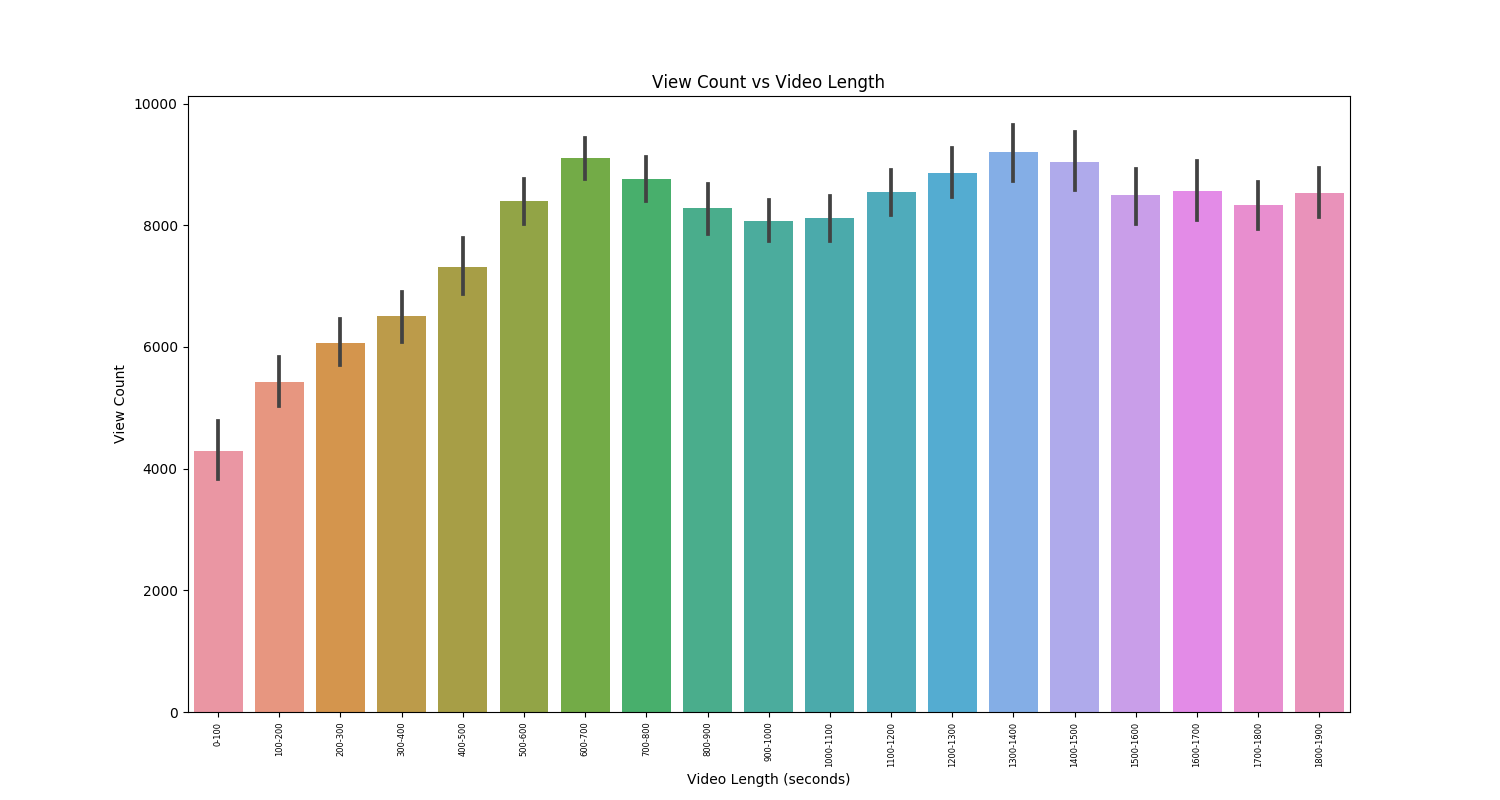
\includegraphics[width=7cm]{images/view_length_bar.png}
% \caption{Bar plot of view and video length}
% \label{fig:1figsA}}
% \qquad
% \begin{minipage}{5cm}
% 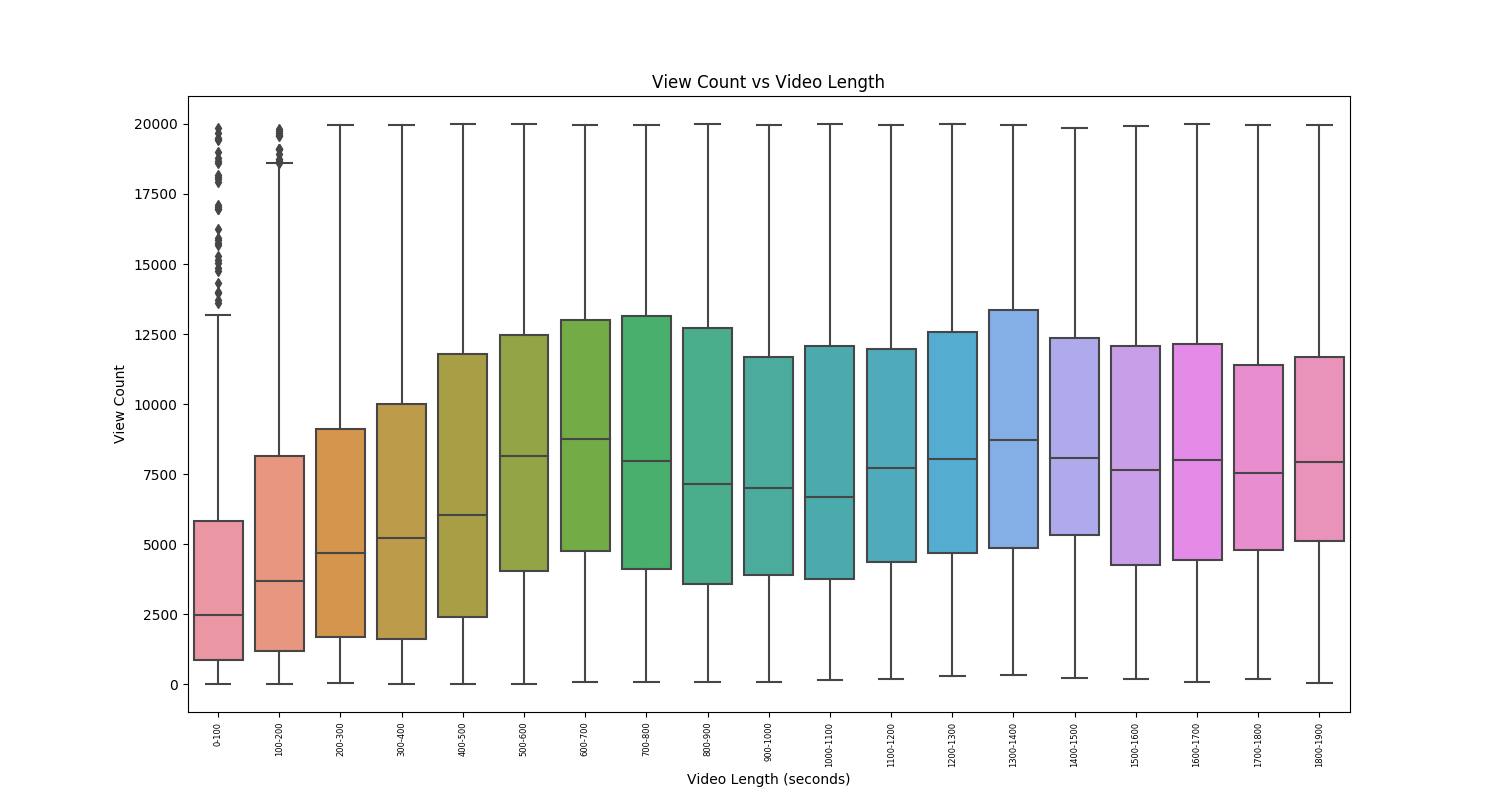
\includegraphics[width=7cm]{images/view_length_box.png}
% \caption{Box plot of view and video length}
% \label{fig:1figsB}
% \end{minipage}
% \end{figure}

\begin{figure}[!htpb]
    \centering
    \subfloat[\centering Bar plot of views and video length]{{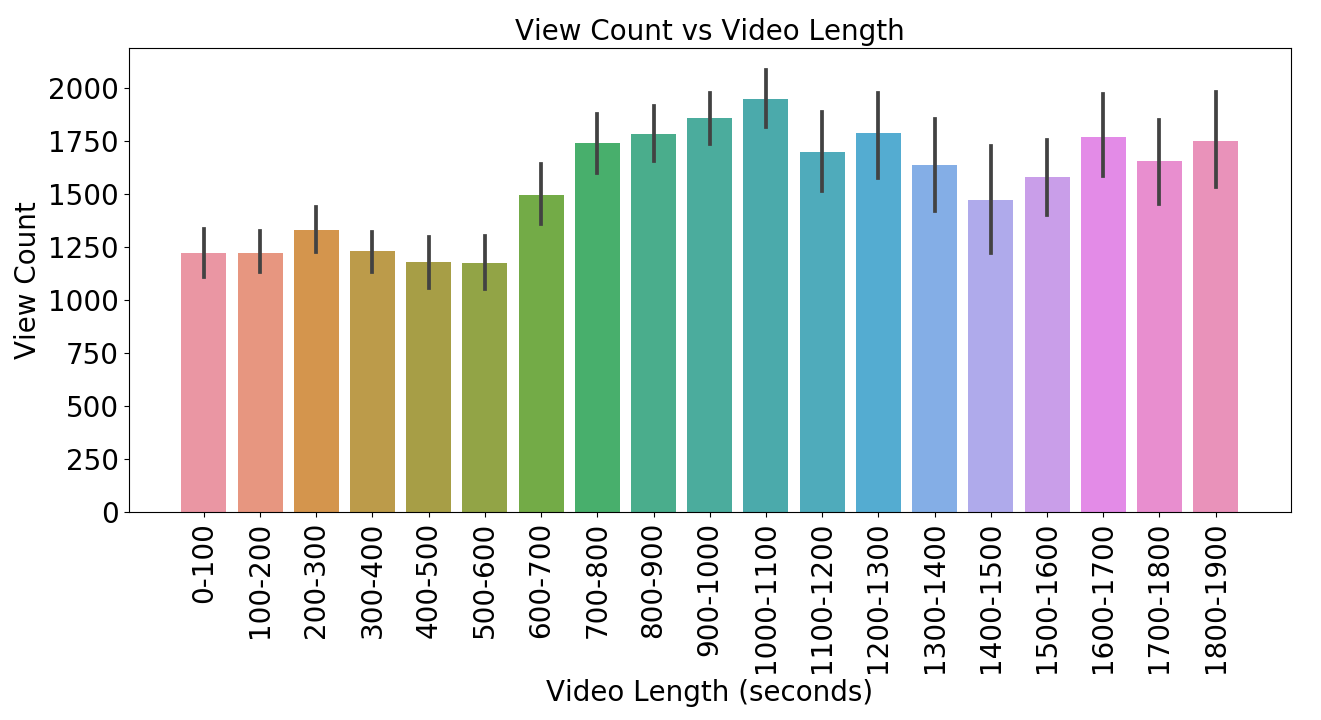
\includegraphics[width=0.49\textwidth]{images/global_optimal_viewCount_bar.png}} \label{fig:views_video_length_1}} \hspace{-2em}%
    \qquad
    \subfloat[\centering Box plot of views and video length]{{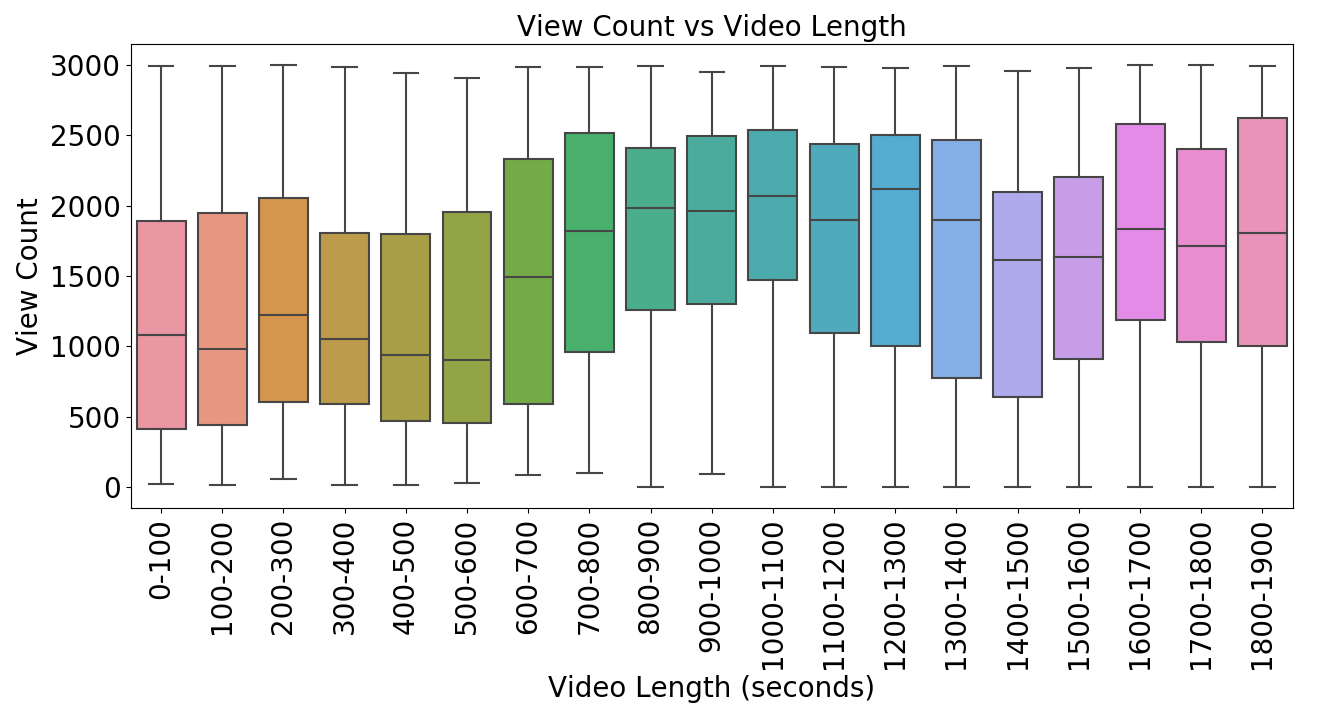
\includegraphics[width=0.49\textwidth]{images/global_optimal_viewCount.png}}\label{fig:views_video_length_2}}%
    % \caption{Box plot of view and video length}%
    
    \caption{Variation of views with video length}%
\end{figure}
\FloatBarrier

% 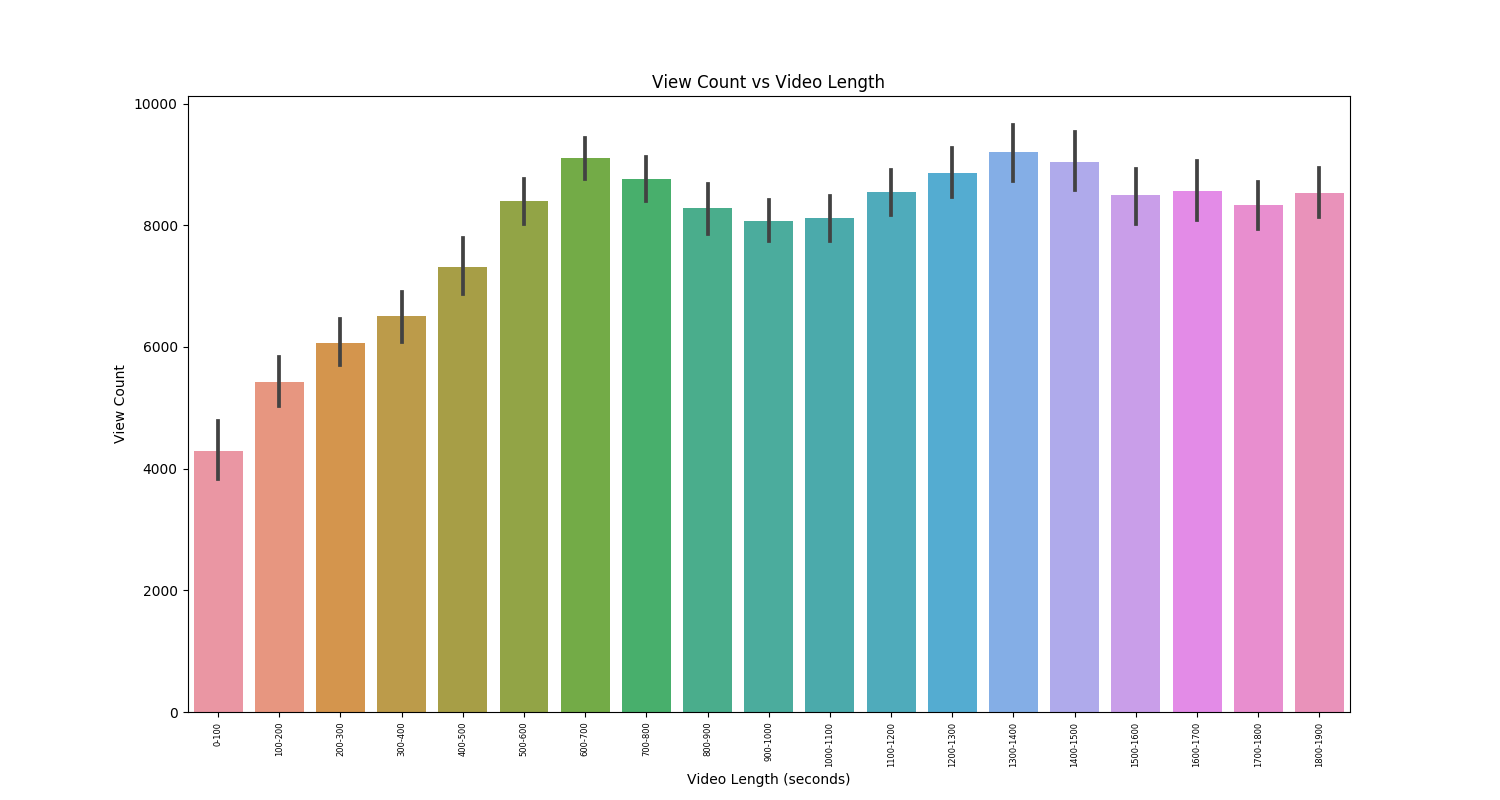
\includegraphics[width=16cm, height=10cm]{images/view_length_bar.png}\\
% Fig : Bar plot of view count vs video length

\noindent We also used the box plot to depict groups of numerical data through their quartiles graphically.

% 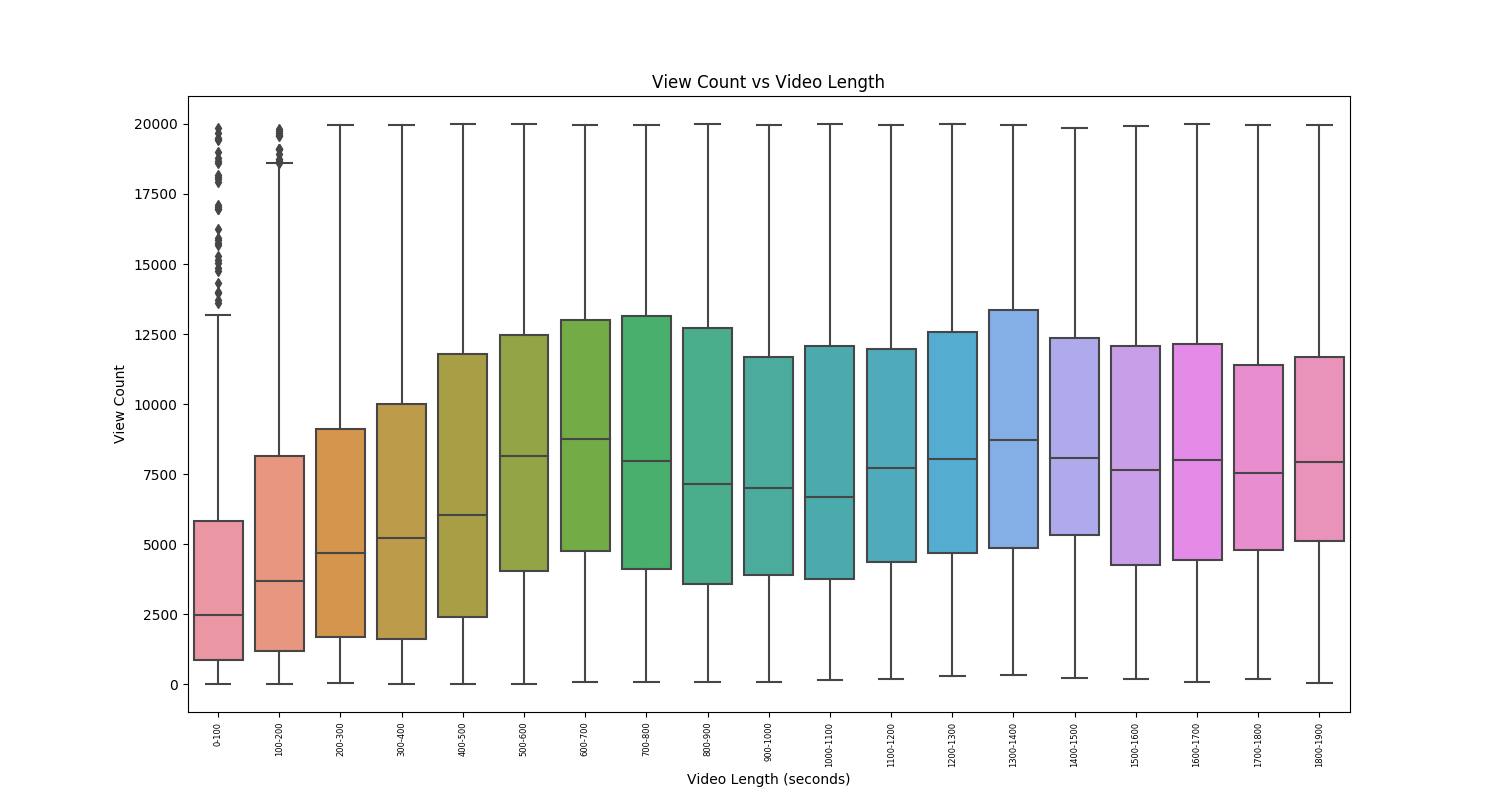
\includegraphics[width=16cm, height=10cm]{images/view_length_box.png}\\
% Fig : Box plot of view count vs video length

\noindent We observed that although the shorter videos fared badly with reference to the views they were able to attract, the views increased rapidly with an increase in length. We observed peaks around the \textbf{10 minute} mark and  \textbf{25 minute} mark. We also observed that videos longer than \textbf{10 minutes} gathered considerably more views than shorter videos. 

% \noindent We believe a viewer prefers to watch videos with length greater than 10 minutes for educational content. Since, it's difficult to actually teach and grasp anything in videos smaller than that.  (NEED TO BE REFINED: SNEHAL). The constant trend for videos with length greater than 10 minutes can again be attributed to this. 

We attribute the preference to longer videos with the inherent abstrusity of educational content. Moreover, in contrast to content comedy/gaming/entertainment content, we didn't observe any negative trend with respect to increasing video length. 

\subsubsection{Likes and Comments}
We also drew a correlation of analytical metrics like likes on the video or the number of comments on a video with the video length (see figures 3 and 4).

We observe a peak for educational videos with length around \textbf{10 minutes}, but the like and comment count gradually decreases with increasing video length. We observed steep decrease in the metrics at around \textbf{15 minute mark}, \textbf{20 minute mark} and \textbf{25 minute mark}.

This shows that even though videos longer than 10 minutes help increase the number of clicks to the videos, having longer videos decreases the number of likes and comments, which to some extent shows a dip in user satisfaction.
% \begin{figure}[hbt!]
% \centering
% \parbox{7cm}{
% 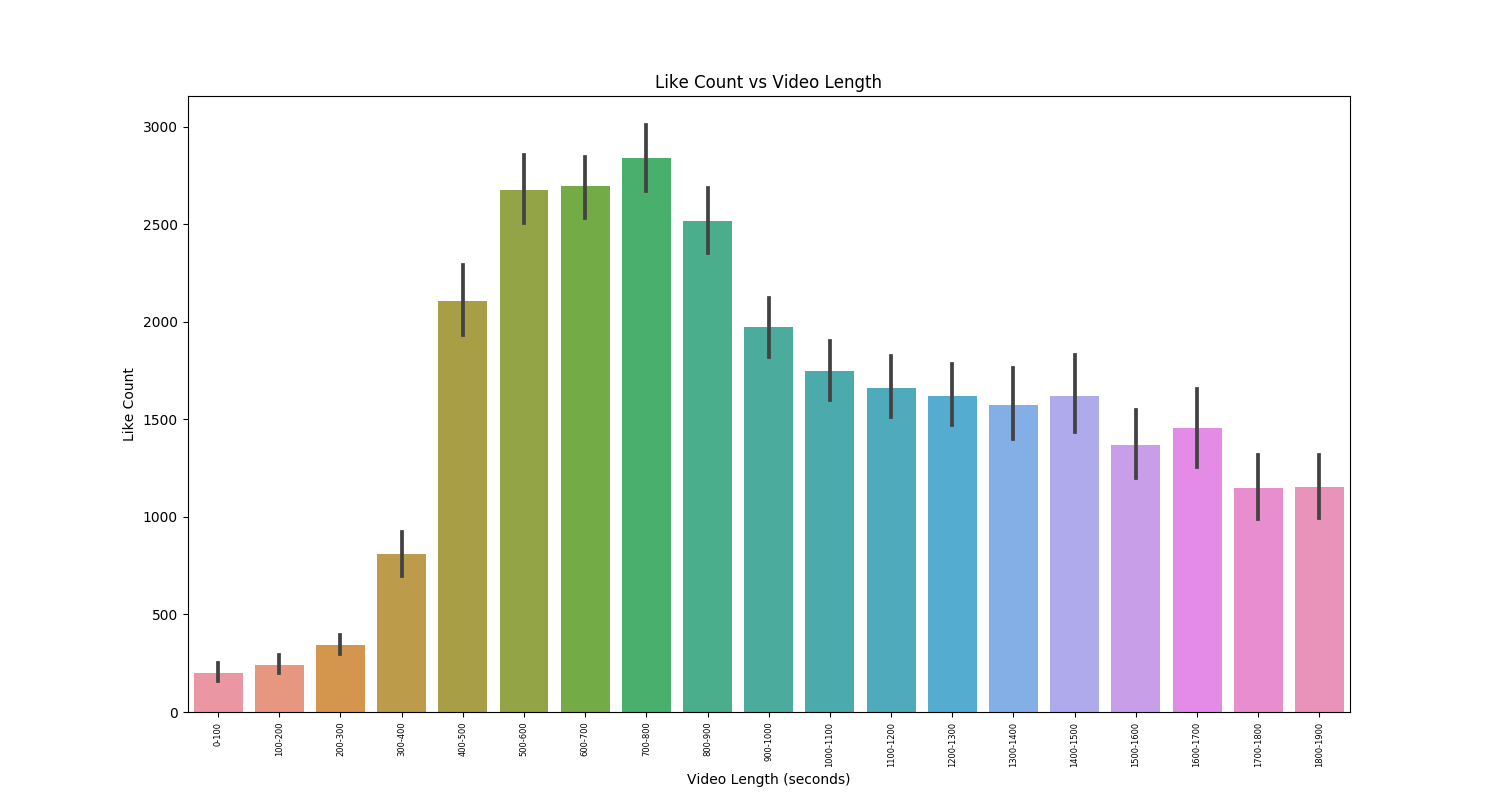
\includegraphics[width=7cm]{images/like_length_bar.png}
% \caption{Bar plot of like and video length}
% \label{fig:2figsA}}
% \qquad
% \begin{minipage}{5cm}
% 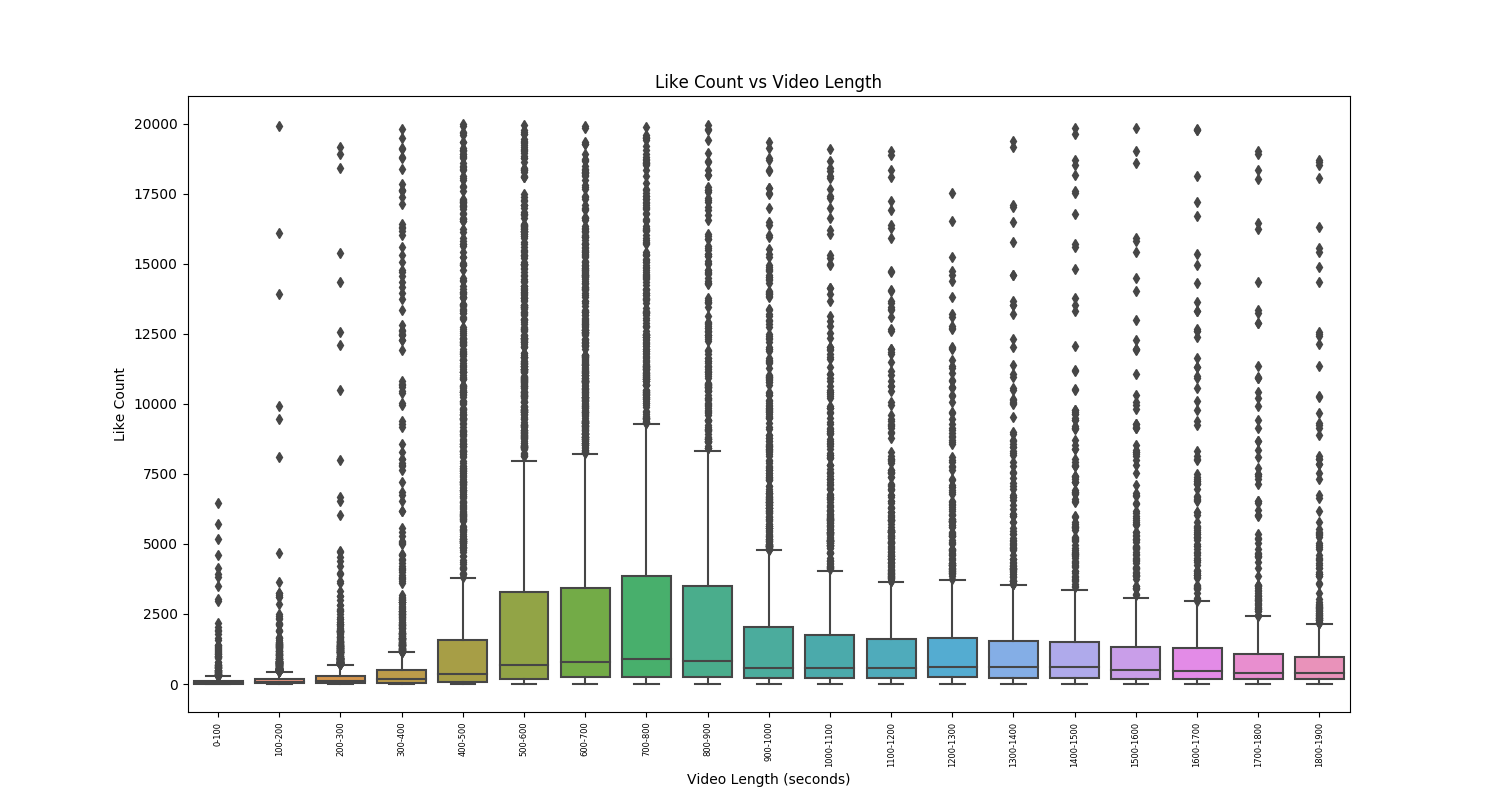
\includegraphics[width=7cm]{images/like_length_box.png}
% \caption{Box plot of like and video length}
% \label{fig:2figsB}
% \end{minipage}
% \end{figure}

\begin{figure}[!htpb]
    \centering  
    \subfloat[\centering Bar plot of likes vs video length]{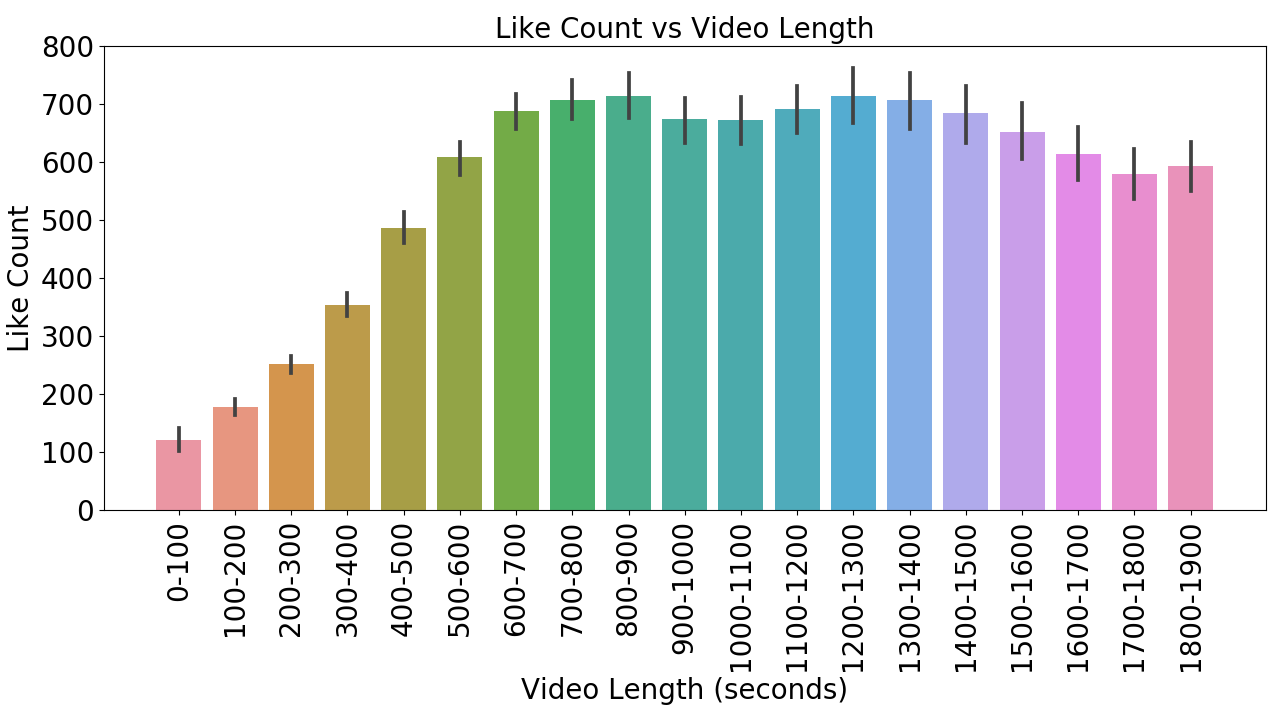
\includegraphics[width=0.49\textwidth]{images/global_optimal_likeCount_bar.png}\label{fig:likes_video_length_1}} \hspace{-2em}%
    \qquad
    \subfloat[\centering Box plot of likes vs video length]{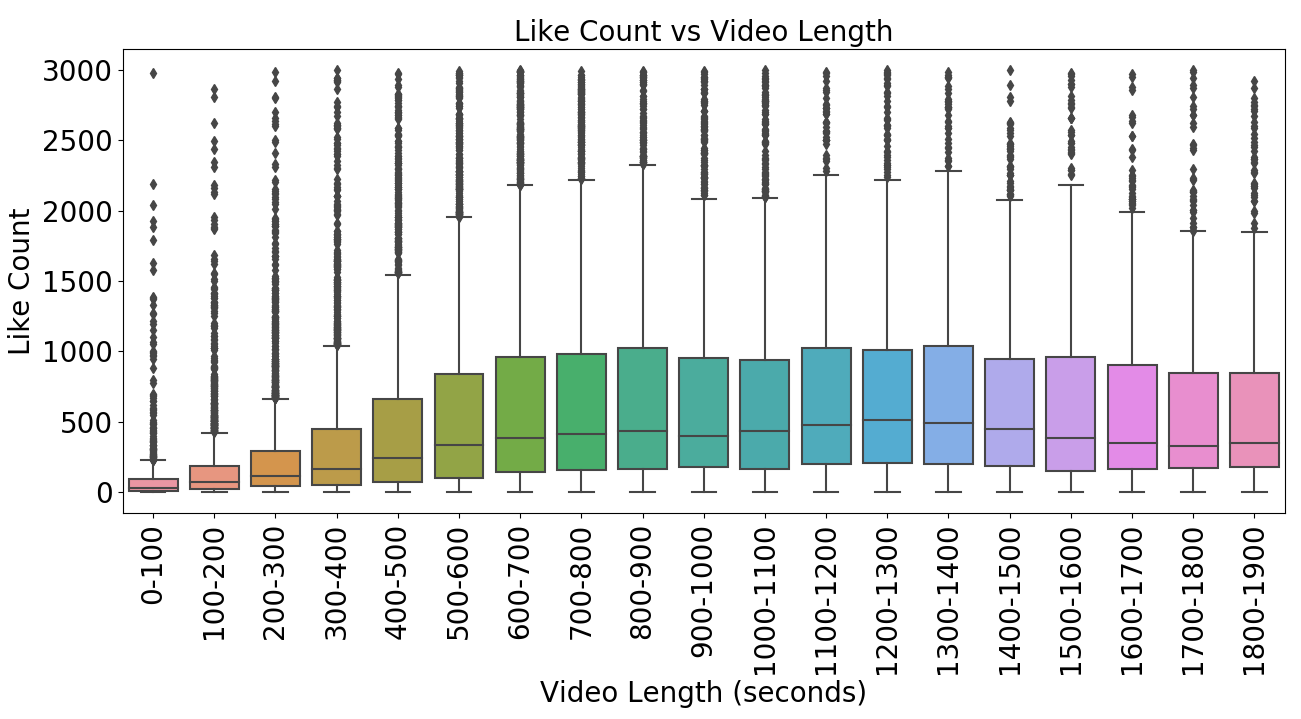
\includegraphics[width=0.49\textwidth]{images/global_optimal_likeCount.png}\label{fig:likes_video_length_2}} \\%
    \caption{Variation of count of likes with Video Length}
    % \caption{Box plot of view and video length}%
    %
\end{figure}
\FloatBarrier

% \begin{figure}[hbt!]
% \centering
% \parbox{7cm}{
% 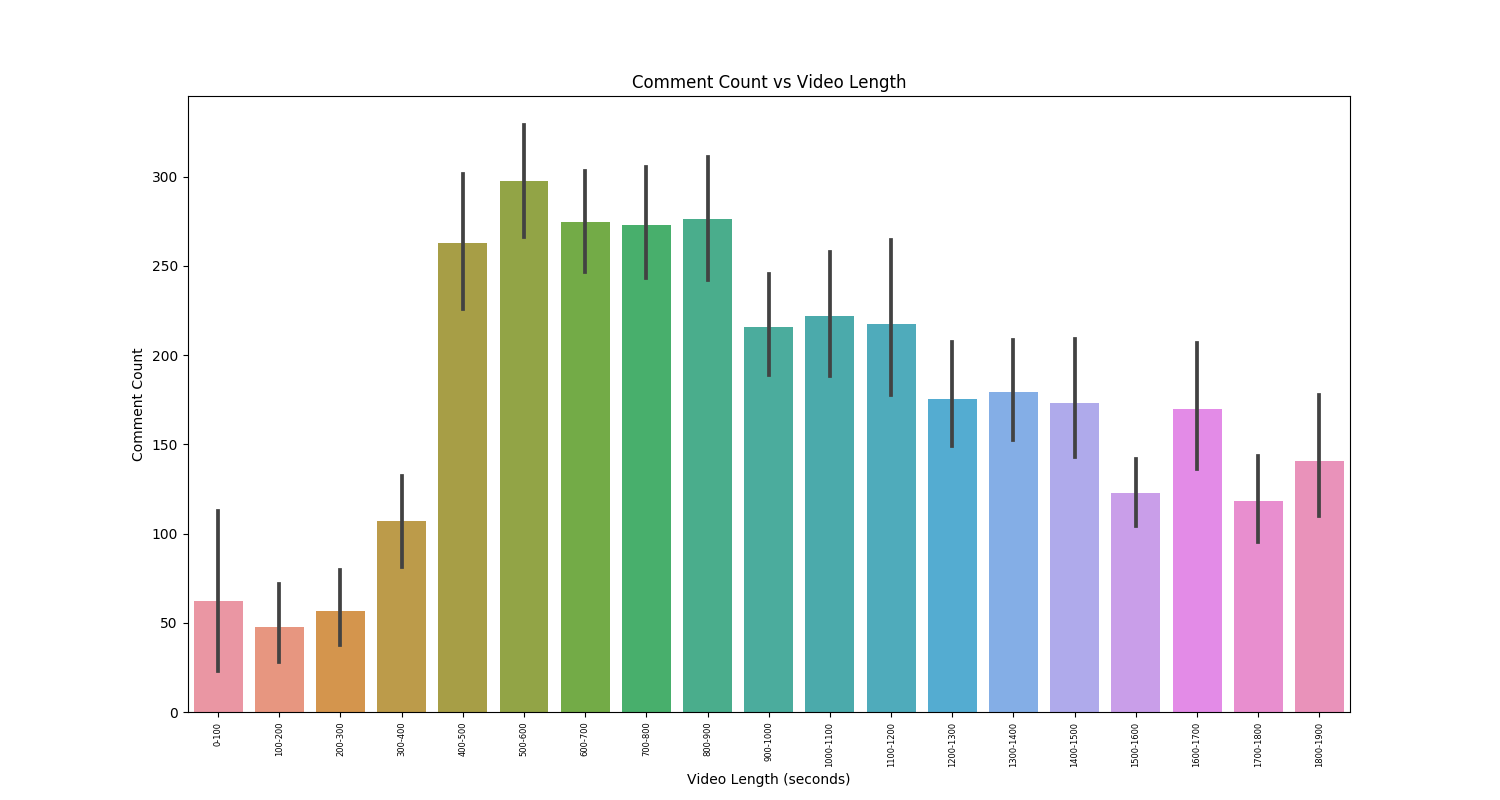
\includegraphics[width=7cm]{images/comment_length_bar.png}
% \caption{Bar plot of comment and video length}
% \label{fig:2figsA}}
% \qquad
% \begin{minipage}{5cm}
% 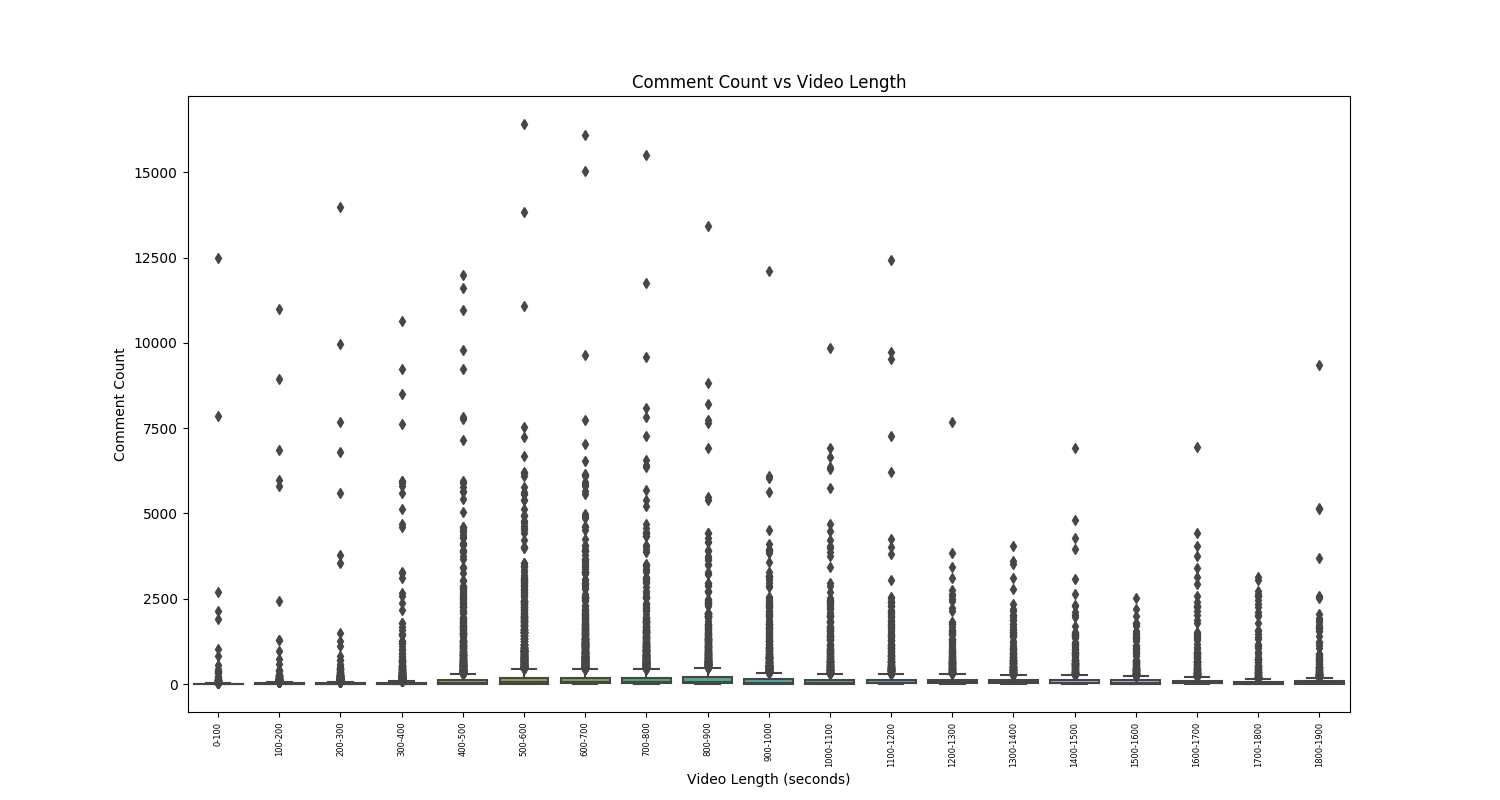
\includegraphics[width=7cm]{images/comment_length_box.png}
% \caption{Box plot of comment and video length}
% \label{fig:2figsB}
% \end{minipage}
% \end{figure}

\begin{figure}[!htpb]
    \centering
    \subfloat[\centering Bar plot of comments vs video length]{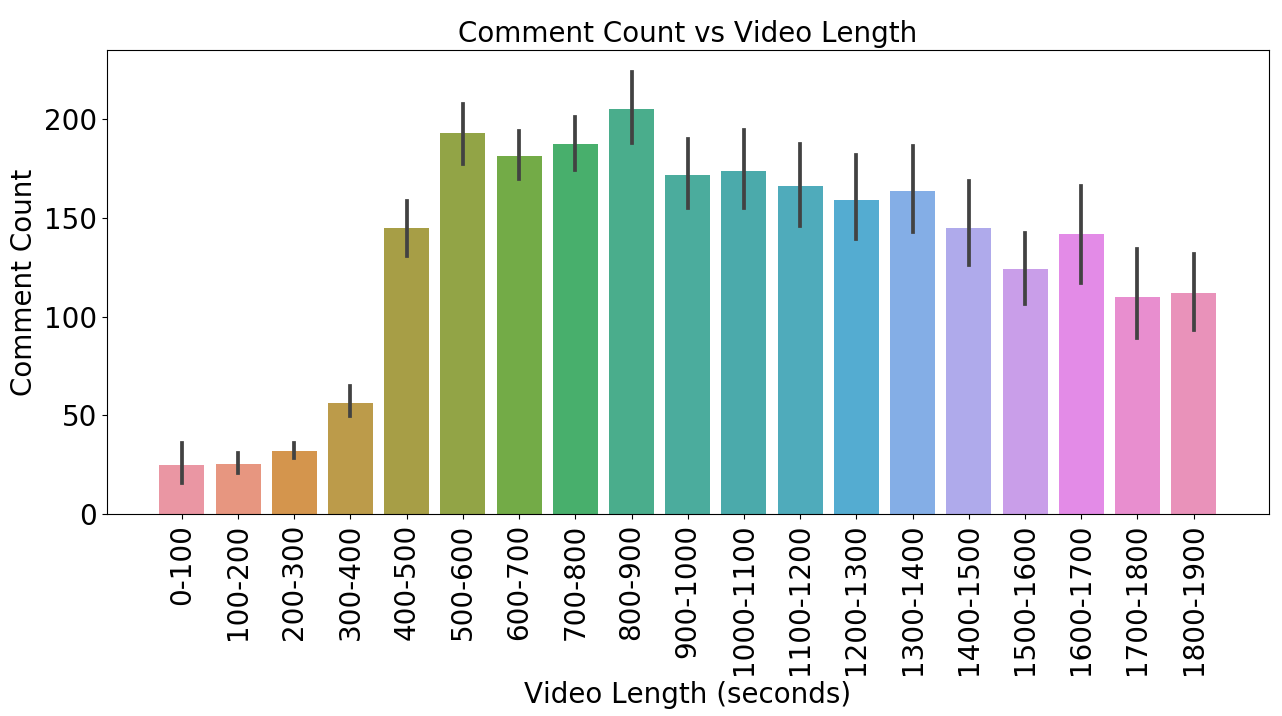
\includegraphics[width=0.49\textwidth]{images/global_optimal_commentCount_bar.png}\label{fig:comment_video_length_1}} \hspace{-2em}%
    \qquad
    \subfloat[\centering Box plot of comments vs video length]{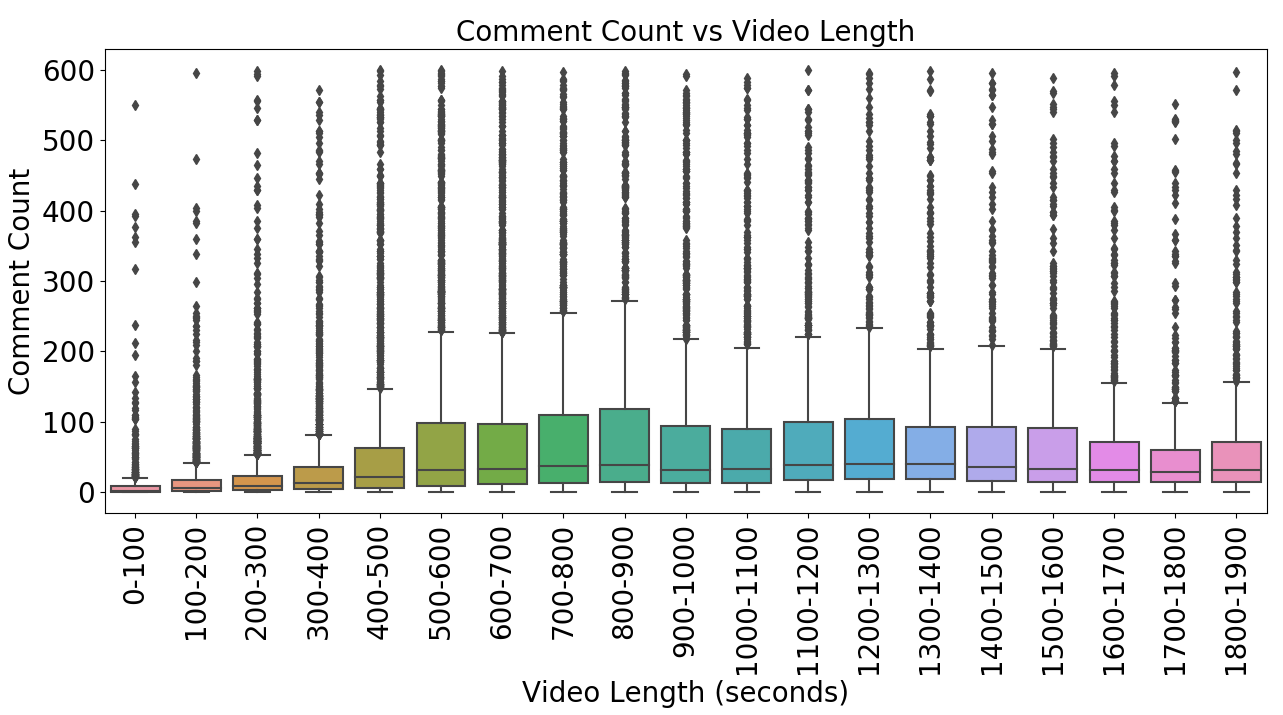
\includegraphics[width=0.49\textwidth]{images/global_optimal_commentCount.png}\label{fig:comment_video_length_2}}\\%
    % \caption{Box plot of view and video length}%
    \caption{Variation of count of comments with Video Length}
    \label{fig:comment_video_length}%
\end{figure}
\FloatBarrier
\subsection{Correlation between Frequency of Likes, Views and Comments}
\label{correlation}
\begin{figure}[!htpb]
    \centering
    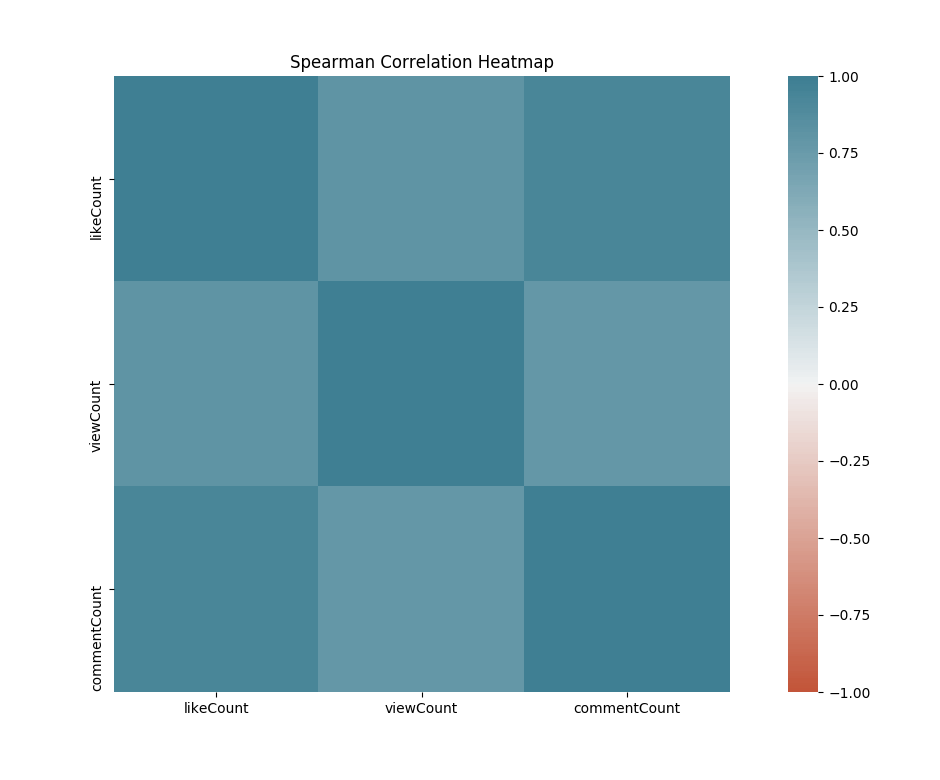
\includegraphics[width=9cm]{images/correlation_heatmap.png}%
    \caption{Spearman Correlation Heatmap between LikeCount, ViewCount, and CommentCount}
    % \caption{Box plot of view and video length}%
    \label{fig:spearman}%
\end{figure}

We see a strong positive correlation between all the pairs of variables. This is slightly different from other content types such as comedy/gaming/entertainment, where highly disliked videos also gather a large number of views (Figure \ref{fig:spearman}).

\subsection{College Ranking Analysis}
\label{collge_rank}
To analyze the college wise distribution of educational content, we filtered videos for the top 5 universities according to QS world university ranking 2021. These were IIT Kanpur, IIT Madras, IIT Bombay, IIT Delhi, and IIT Kharagpur from NPTELHRD channel.

We then proceeded with accumulating the branch wise data distribution of the same and took four branches into consideration, namely Computer Science \& Engineering (CSE), Electrical Engineering (EE), Mechanical Engineering (ME) and Chemical Engineering (CHE) (Figure \ref{fig:branch_video_counts}). We collected data for each channel's number of videos, and three evaluation metrics, namely average likes, average views, and the like/dislike ratio.
% (JUST A ROUGH DESCRIPTION. NEEDS MODIFICATION. UMANG, KESHAV, AYUSH, SNEHAL)

\begin{figure}[!htpb]
    \centering
    
    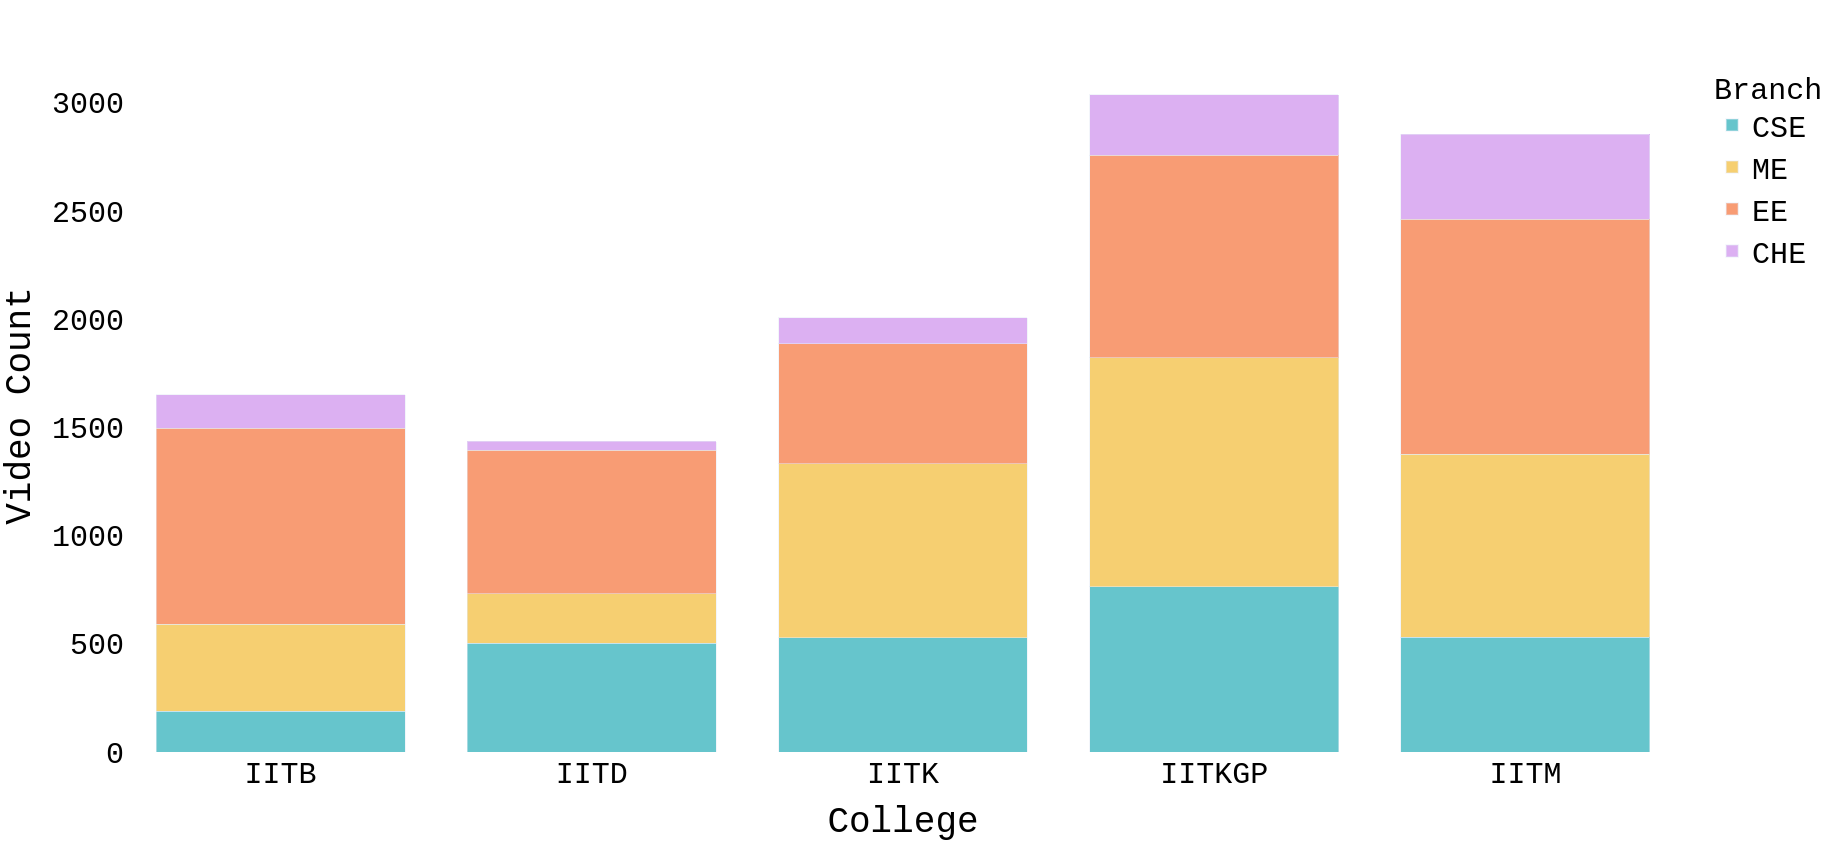
\includegraphics[width=15cm]{images/video_counts.png}%
    \caption{Branchwise NPTEL Videos for each college}
    % \caption{Box plot of view and video length}%
    \label{fig:branch_video_counts}%
\end{figure}






\subsubsection{Comparison with QS rankings}

We tried to derive correlations between the data we collected and the QS World University Rankings (see table \ref{qs_ranking}). We found that channels with better ranks had greater average views on their channels. However, when it came to actually interacting with the content in terms of likes and comments, we observed that other universities fared better.

For example, we observed the IIT Bombay has the highest average views when considering the videos related to the CSE department and IIT Delhi had the highest average views related to EE department videos, however when we observed the like/dislike ratio for both CSE and EE departments, we found IIT Kanpur to perform better.
\begin{table}[!htpb]
\parbox{.44\linewidth}{
\centering
\begin{tabular}{|c|c|}
\hline
University    & QS University Rankings 2021 \\ \hline
IIT Bombay    & Ranked 172          \\
IIT Delhi     & Ranked 193           \\
IIT Madras    & Ranked 275          \\
IIT Kharagpur & Ranked 314       \\
IIT Kanpur    & Ranked 350          \\
\hline     

\end{tabular}\vspace{3mm}
\caption{QS World rankings}
\label{qs_ranking}
}
\hfill
\parbox{.44\linewidth}{
\begin{tabular}{|c|c|}
\hline
University    & Overall Average views \\ \hline
\textbf{IIT Delhi}     & \textbf{44962}      \\
IIT Kharagpur & 32303      \\
IIT Bombay    & 28365      \\
IIT Madras    & 28184      \\
IIT Kanpur    & 17723 \\  \hline   
\end{tabular}\vspace{3mm}

\caption{Overall Average views}
}
\end{table}
 
%     \begin{table}[!]
% \begin{center}
% \begin{tabular}{ |c|c|c| c|c|c| } 
%  \hline
%  College & Branch & Video Count &  Average views & Average likes & Like/dislike ratio  \\\hline
%  IITK &  CSE &  528 & 7114.051 &  26.159 & 0.948\\
%  IITD& CSE& 503& 44451.089& 107.056& 0.943\\
%  IITB& CSE& 188& 58259.101& 132.601& 0.939\\
%  IITM& CSE& 530& 42674.226& 123.460& 0.938\\
%  IITKGP& CSE& 764& 38803.469& 92.077& 0.937\\
% \hline
%  IITM& ME& 845& 11474.535& 55.231& 0.964\\
%  IITK& ME& 804& 23718.689& 76.672& 0.962\\
%  IITB& ME& 403& 30586.285& 95.814& 0.960\\
%  IITKGP& ME& 1059& 31227.553& 119.791& 0.957\\
%  IITD& ME& 228& 32261.667& 113.474& 0.940\\
% \hline
%  IITK& EE& 554& 20808.715& 65.722& 0.960\\
%  IITD& EE& 664& 52339.633& 129.443& 0.953\\
%  IITM& EE& 1088& 41959.692& 134.225& 0.953\\
%  IITB& EE& 904& 25270.758& 67.833& 0.944\\
%  IITKGP& EE& 935& 35999.903& 97.142& 0.937\\
% \hline
%  IITB& CHE& 155& 4378.987& 24.690& 0.963\\
%  IITK& CHE& 121& 10061.661& 38.372& 0.962\\
%  IITM& CHE& 392& 6379.497& 34.115& 0.960\\
%  IITKGP& CHE& 280& 6292.718& 22.954& 0.959\\
%  IITD& CHE& 40& 1345.050& 5.025& 0.905\\

% %  128 & 7.63078 \\
% %  256 & 57.0212\\
%  \hline
%  \end{tabular}\vspace{3mm}
% \caption{Branch wise comparison across five IITs}
% \end{center}
% \end{table}
% \begin{table}[!htpb]
% \begin{center}
% \begin{tabular}{|c|c|}
% \hline
% University    & QS World University Rankings 2021 \\ \hline
% IIT Bombay    & Ranked 172          \\
% IIT Delhi     & Ranked 193           \\
% IIT Madras    & Ranked 275          \\
% IIT Kharagpur & Ranked 314       \\
% IIT Kanpur    & Ranked 350          \\
% \hline     
% \end{tabular}\vspace{3mm}
% \caption{QS World rankings}
% \label{qs_ranking}
% \end{center}
% \end{table}

% \begin{table}[!htpb]
% \begin{center}
% \begin{tabular}{|c|c|}
% \hline
% University    & Overall Average views \\ \hline
% \textbf{IIT Delhi}     & \textbf{44962.98}      \\
% IIT Kharagpur & 32303.39      \\
% IIT Bombay    & 28365.15      \\
% IIT Madras    & 28184.32      \\
% IIT Kanpur    & 17723.73 \\  \hline   
% \end{tabular}\vspace{3mm}
% \caption{Overall Average views}
% \end{center}
% \end{table}


\begin{table}[!htpb]
\parbox{.40\linewidth}{
\centering
 \begin{tabular}{ |p{1.5em}|p{2em}|p{2em}|p{2em}|p{2em}|p{2.7em}| } 
 \hline
  & IITB & IITD &  IITK & IITM & IITKGP  \\\hline
  CSE & \textbf{58259} & 44451 & 7114 & 42674 & 38803\\
  EE & 25270 &  \textbf{52339} &20808 & 41959 & 35999\\
  ME & 30581 & \textbf{32261} & 23718 & 11474 & 31227\\
  CHE &4378 & 1345 & \textbf{10061} &6379 & 6292\\
 \hline
 \end{tabular}\vspace{3mm}

\caption{Table for Average Views}
}
\hfill
\parbox{.40\linewidth}{
\centering
\hspace{-3em} \begin{tabular}{|p{1.5em}|p{1.7em}|p{1.7em}|p{1.7em}|p{1.7em}|p{2.7em}|} 
 \hline
  & IITB & IITD &  IITK & IITM & IITKGP  \\\hline
  CSE & 93.9 & 94.3 & \textbf{94.8} & 93.8 & 93.7\\
  EE & 94.4 &  95.3 & \textbf{96.0} & 95.3 & 93.7\\
  ME & 96 & 94 & 96.2 & \textbf{96.4} & 95.7\\
  CHE & \textbf{96.3} & 90.5 & 96.2 & 96 & 95.9\\

 \hline
 \end{tabular}\vspace{3mm}
\caption{Table for like percentage}
}
\end{table}


% \begin{table}
% \begin{center}
% \begin{tabular}{ |c|c|c|c|c|c| } 
%  \hline
%   & IITB & IITD &  IITK & IITM & IITKGP  \\\hline
%   CSE & \textbf{33173.0}& 8281.0 & 2654.0 & 20233.0 & 16921.0\\
%   EE & 11400.0 &  \textbf{28339.5} &12296.0 & 15035.0& 18511.0\\
%   ME & 9737.0 & \textbf{16559.5} & 3448.0& 4196.0 & 10778.0\\
%   CHE &2525.0 & 786.0 & \textbf{7204.0} &3046.5 & 1505.0\\
%  \hline
%  \end{tabular}\vspace{3mm}
% \caption{Table for Median views}
% \end{center}
% \end{table}

\newpage
\subsection{Playlist Retention}
We performed viewer retention analysis on the Youtube API. We observed a decline in the views as the playlist progresses

We also perform retention analysis between channels with High school/JEE content (Khan Academy, Unacademy) and channels with college-level content (NPTEL/MIT OCW)

% \begin{figure}[H]
%     \centering
%     \subfloat[\centering NPTEL and MIT OCW ]{{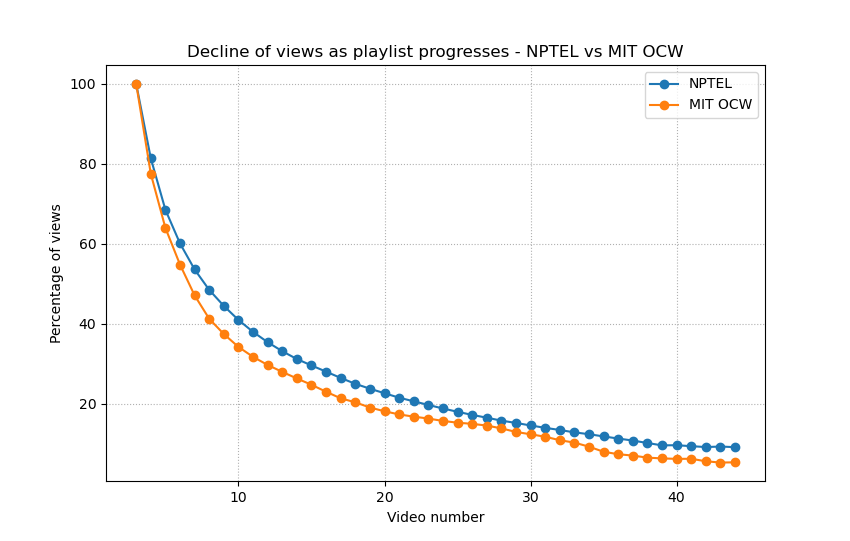
\includegraphics[width=16cm, height=10cm]{images/retention_nptel_vs_mit.png}}}%
% \end{figure}
% \begin{figure}[H]
%     \subfloat[\centering College and JEE channels]{{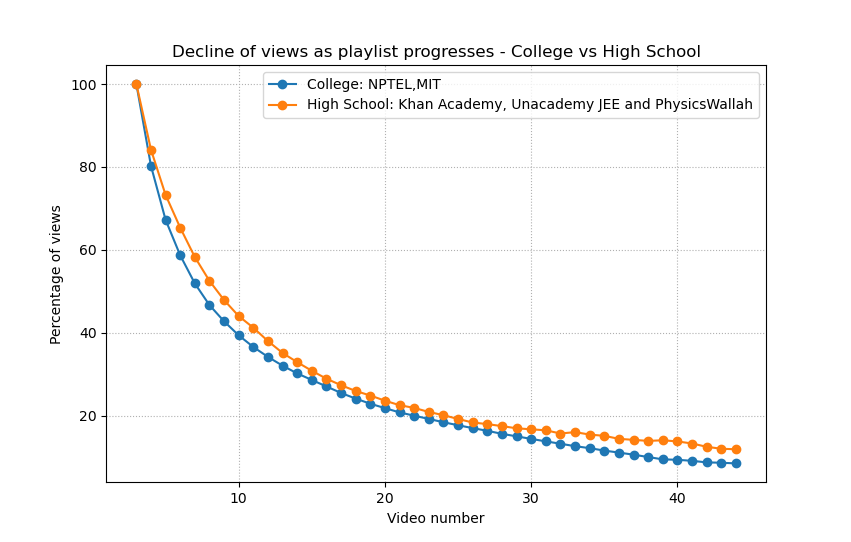
\includegraphics[width=16cm, height=10cm]{images/retention_college_vs_jee.png}}}%
%     \caption{Decline of Views Comparison (from 3rd video)}%
%     \label{fig:example}%
% \end{figure}
% \FloatBarrier
\begin{figure}[!htpb]
    \centering
    \hspace*{-2.5em}\subfloat[\centering NPTEL and MIT OCW ]{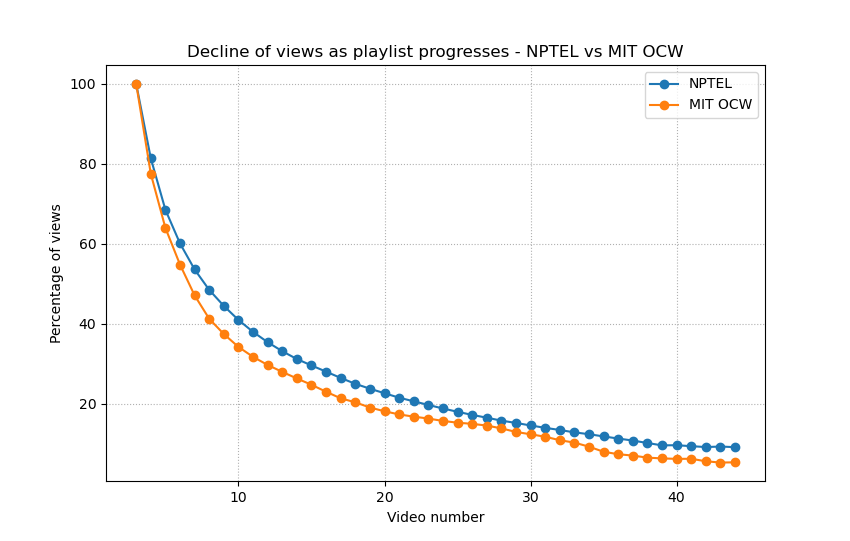
\includegraphics[width=0.59\textwidth]{images/retention_nptel_vs_mit.png} \label{fig:img1}} \hspace*{-4em}
    \qquad
    \subfloat[\centering College and JEE channels]{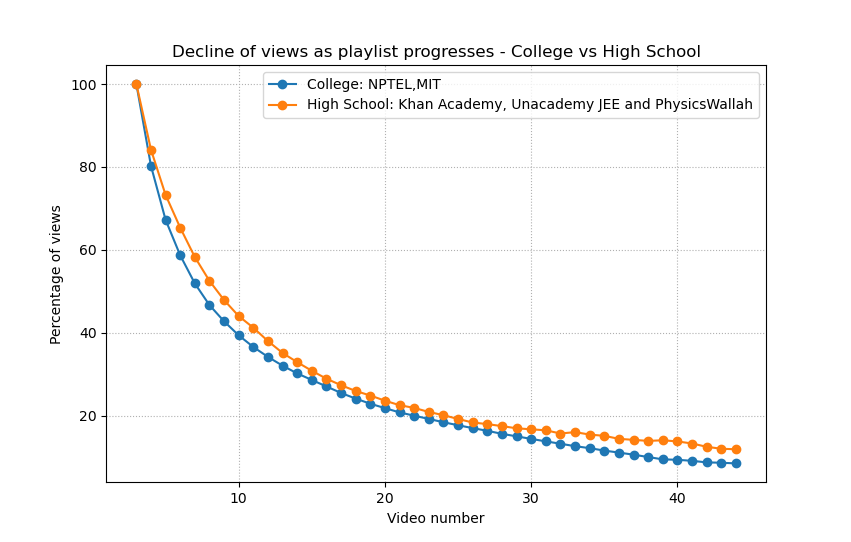
\includegraphics[width=0.59\textwidth]{images/retention_college_vs_jee.png} \label{fig:img2}}\\
    \label{fig:example}%
    \caption{Decline of Views Comparison (from 3rd video)}
\end{figure}
\FloatBarrier

% \begin{figure}[!htpb]
%     \centering
%     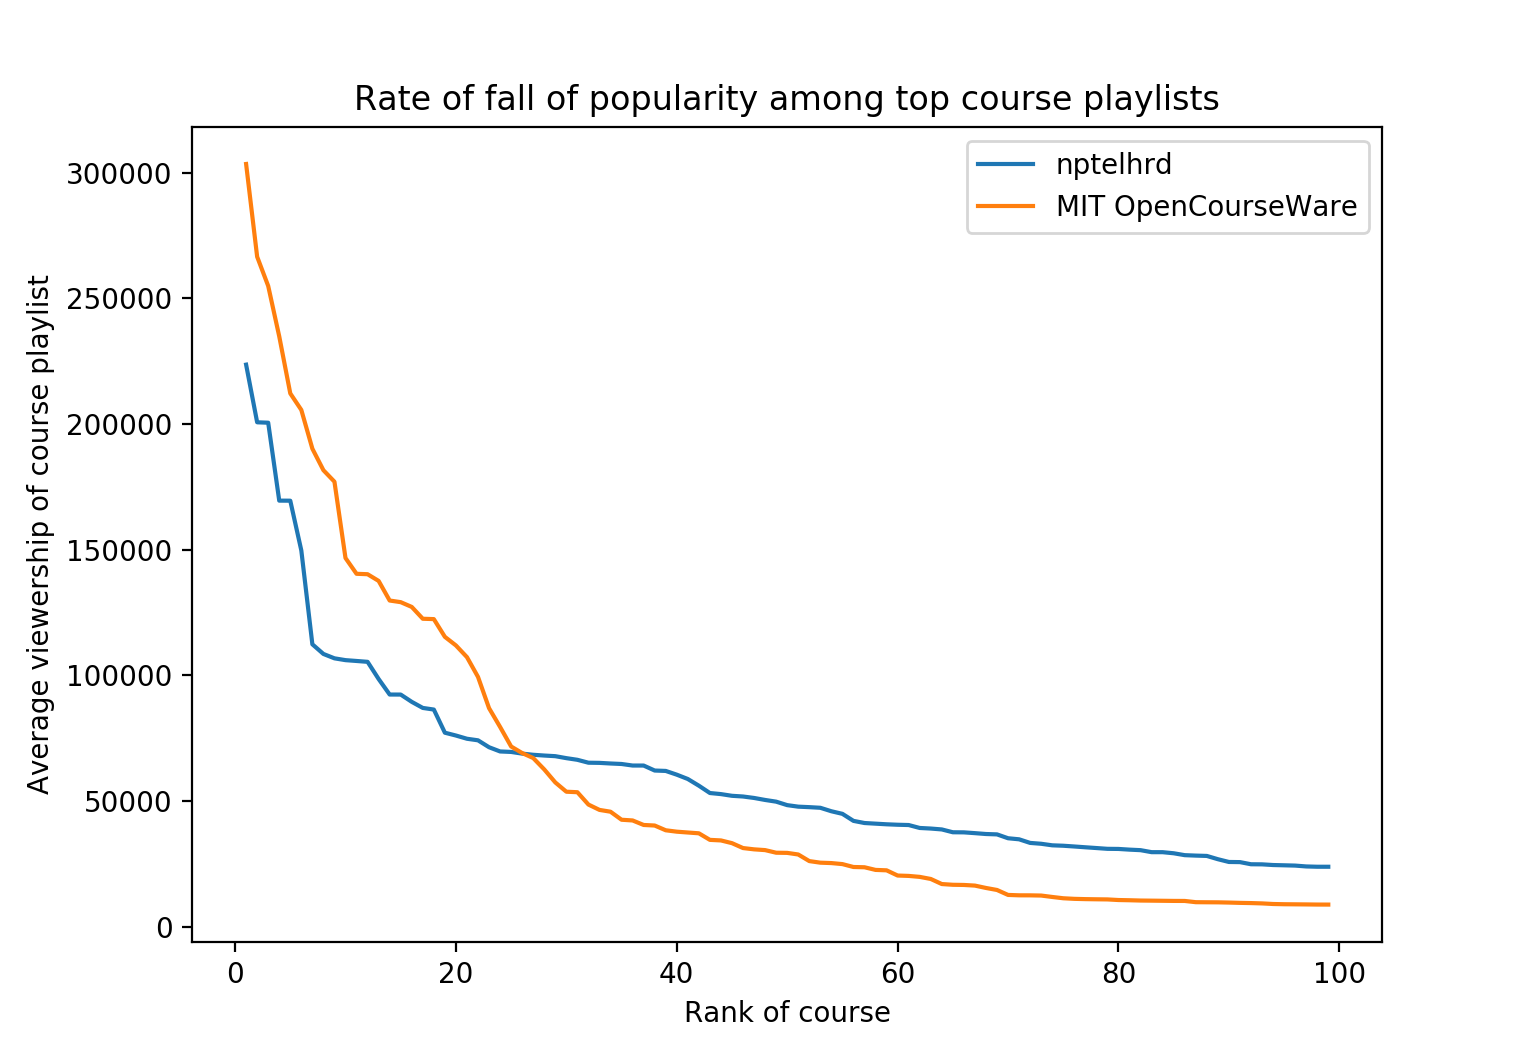
\includegraphics[scale=0.5]{images/fall_of_views.png}
%     \caption{Comparison of fall of popularity among top topics}
%     \label{fig:my_label}
% \end{figure}
% \FloatBarrier

The above graphs provide exciting insights about the retention between channels. We assume that a channel's content has better retention capacity if the decrease in the views with an increase in video numbers is less steep. In the graph, we observe that the viewership of MIT videos decreases more rapidly than the decrease in viewership of NPTEL's videos. Thus, we observe better retention in NPTEL's case.

One possible reason for the increased retention in case of NPTEL can be attributed to the fact that many of the NPTEL courses involve a certification which incentivizes watching videos.

The second graph above shows that the curve for channels with JEE content always remains above the College content curve. This means that the videos/lectures uploaded for university students see a steeper decrease in viewership with the increase in videos.  This is a fascinating result. We believe that this is because of 
\begin{itemize}
\item Target audience for channels with JEE content is the general youtube audience, whereas the target audience for University-based channels are University students. We hypothesize that educational organizations like Khan academy, Unacademy, etc. have focused more on keeping their viewers engaged and consequently on the ease of understanding. In contrast, university-based channels have focus more on delivering lectures and teaching the contents of the course.
\item We also attribute the steeper decrease in viewership for the college-based content to the audience's attention span and diligence. It is possible that a viewer watches the content more seriously on JEE related channels compared to viewers on college content related channels. This can be because high school students are more serious while studying for JEE and watch these videos more thoroughly. Whereas in college, a lot of students develop a more care-free attitude and thus are less motivated.

\end{itemize}

% \newpage
\subsection{Ranking of topics}
\label{topics_ranking}
% \subsubsection{By views}
% Using the playlist data we obtained for the channels \textbf{NPTELHRD} and \textbf{MIT OpenCourseWare}, we create a ranking of the most popular playlist courses. This involved two steps:
% \begin{enumerate}
%     \item Clustering of Topics: Playlist Titles were clustered into topics (where multiple similar playlist titles were grouped into one single topic) using similarity matching and POS-Tagging. Usually, one clustered topic contained playlist courses created for different iterations of the course or other courses with similar content.\\
%     \item Ranking based on views: We then used max aggregation to get the average views for each topic by aggregating the average views of the individual playlist courses for that topic. This resulted in the ranklist as shown below.\\
% \end{enumerate}

\noindent The topics generated after clustering (as explained in section \ref{method_ranking_topics}) are then ranked based on the average viewership. Below are some ranking tables and the statistical graphs that we obtained:

\begin{table}[!htpb]
    \centering
    \begin{tabular}{|c|c|c|c|c|}
    \hline
        \textbf{Rank} & \textbf{Topic} & \textbf{Department} & \textbf{Avg Views} & 
        % \textbf{Avg Likes} & \textbf{Avg Disikes} & \textbf{Avg Comments} & 
        \textbf{\#Videos}\\
    \hline
        1 & Fundamentals of Operations Research & Mechanical & 223591 & 22\\
        2 & Basic Electrical Technology & Electrical & 200650 & 39\\
        3 & Design of Reinforced Concrete Structures & Civil & 200482 & 70\\
        4 & Basic Electrical Circuits & Electrical & 169476 & 101\\
        5 & Data Structures and Algorithms & Computer Science & 169452 & 36\\
        6 & Thermodynamics & Mechanical & 149631 & 72\\
        7 & Programming and Data Structure & Computer Science & 112309 & 32\\
        8 & Advanced Operations Research & Mechanical & 108464 & 39\\
        9 & Convective Heat and Mass Transfer & Mechanical & 106719 & 122\\
        10 & Biochemistry I & Biotechnology & 105999 & 28\\
    \hline
    \end{tabular}\vspace{3mm}
    \caption{Top 10 popular NPTEL topics}
    \label{tab:my_label}
\end{table}
\Floatbarrier

\begin{table}[!htpb]
    \centering
    \begin{tabular}{|c|c|c|c|c|}
    \hline
        \textbf{Rank} & \textbf{Topic} & \textbf{Department} & \textbf{Avg Views} & 
        % \textbf{Avg Likes} & \textbf{Avg Disikes} & \textbf{Avg Comments} & 
        \textbf{\#Videos}\\
    \hline
        \multirow{2}{*}{1} & Introduction to Computer Science \& & \multirow{2}{*}{Computer Science} & \multirow{2}{*}{384292} & \multirow{2}{*}{100}\\
        & Programming in Python & & &\\
        2 & Linear Algebra & Mathematics & 303443 & 110\\
        3 & Introduction to Probability & Mathematics & 266535 & 313\\
        4 & Listening, Speaking & English & 254899 & 4\\
        \multirow{2}{*}{5} & Topics in Mathematics \& & \multirow{2}{*}{Mathematics} & \multirow{2}{*}{234844} & \multirow{2}{*}{24}\\
        & Applications in Finance & & &\\
        6 & Quantum Physics III & Physics & 212147 & 266\\
        7 & Artificial Intelligence & Computer Science & 205565 & 30\\
        \multirow{2}{*}{8} & Introduction to Computational Thinking & \multirow{2}{*}{Computer Science} & \multirow{2}{*}{190149} & \multirow{2}{*}{15}\\
        & \& Data Science & & &\\
        9 & Single Variable Calculus & Mathematics & 181583 & 35\\
        10 & H/W Help for Multivariable Calculus & Mathematics & 177010 & 192\\
        
    \hline
    \end{tabular}\vspace{3mm}
    \caption{Top 10 popular MITOCW topics}
    \label{tab:my_label}
\end{table}
\Floatbarrier

\begin{figure}[!htpb]
    \centering
    \hspace*{-2.5em}\subfloat[\centering Views distribution for NPTEL topics]{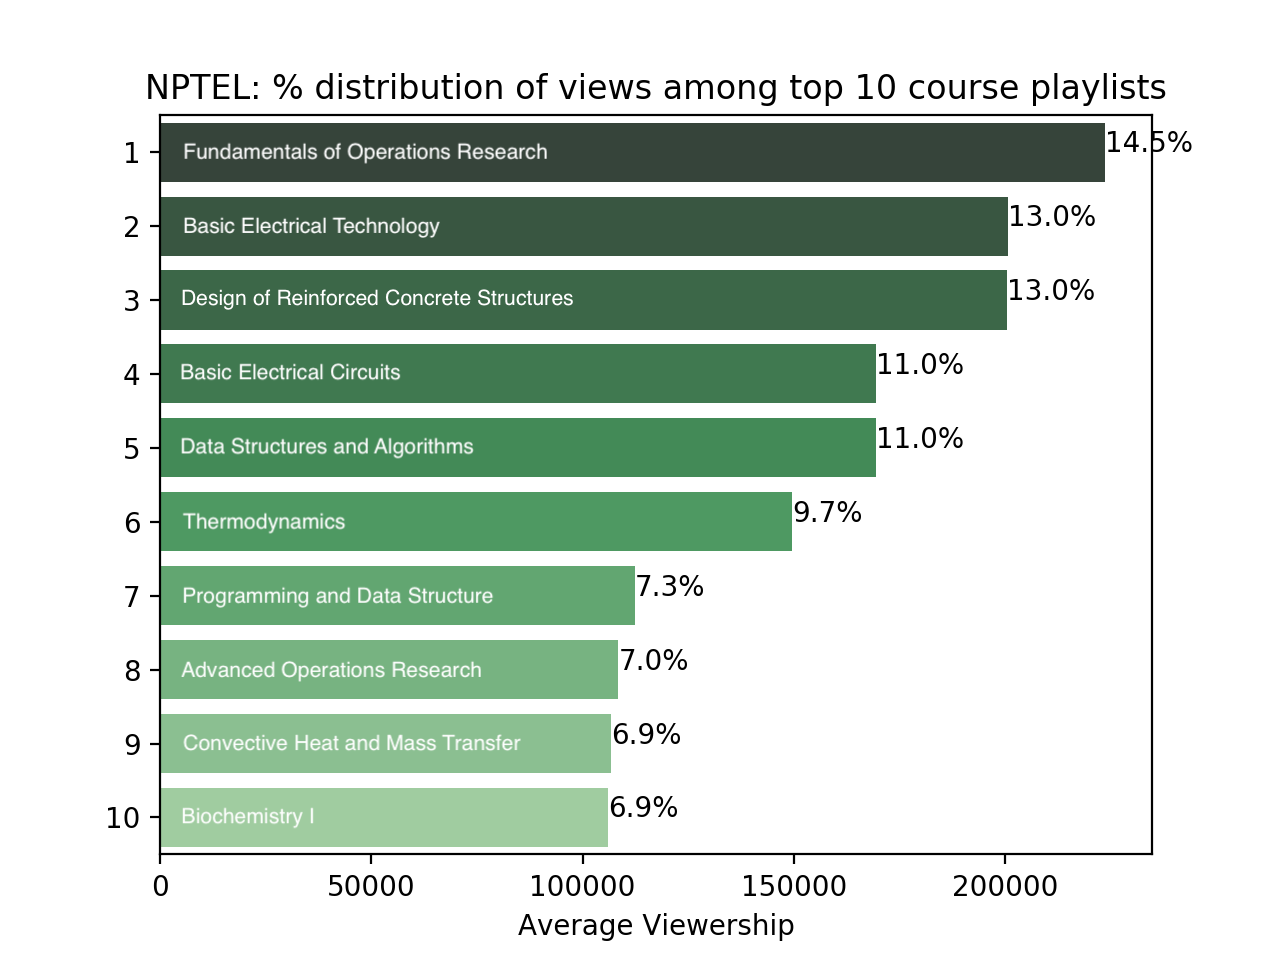
\includegraphics[width=0.59\textwidth]{images/nptel_views_distr.png} \label{fig:img1}} \hspace*{-4em}
    \qquad
    \subfloat[\centering Views distribution for MITOCW topics]{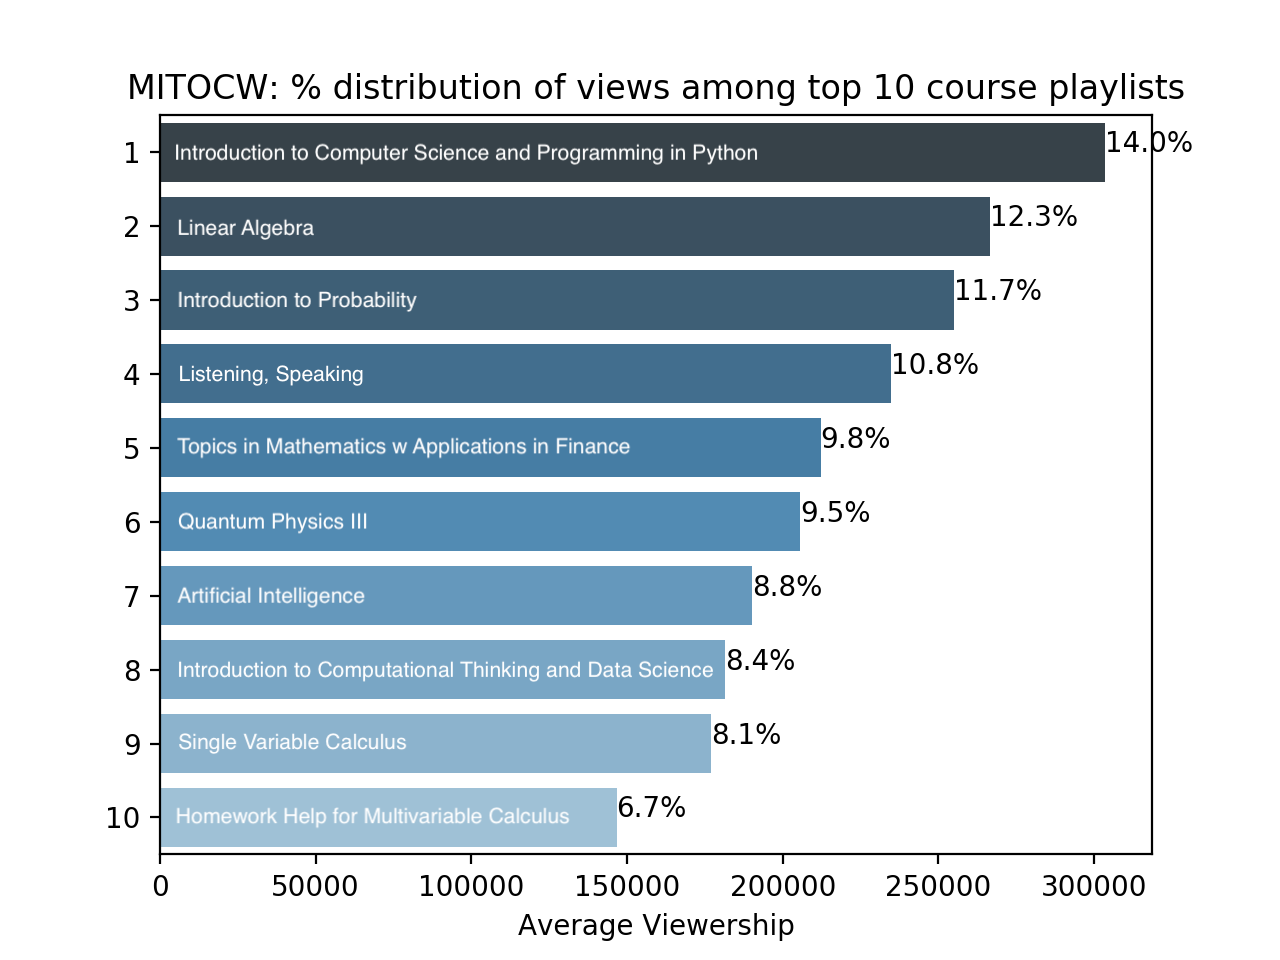
\includegraphics[width=0.59\textwidth]{images/mitocw_views_distr.png} \label{fig:img2}}\\
    \label{fig:example}%
    \caption{Views distribution comparison}
\end{figure}
\FloatBarrier

\begin{figure}[!htpb]
    \centering
    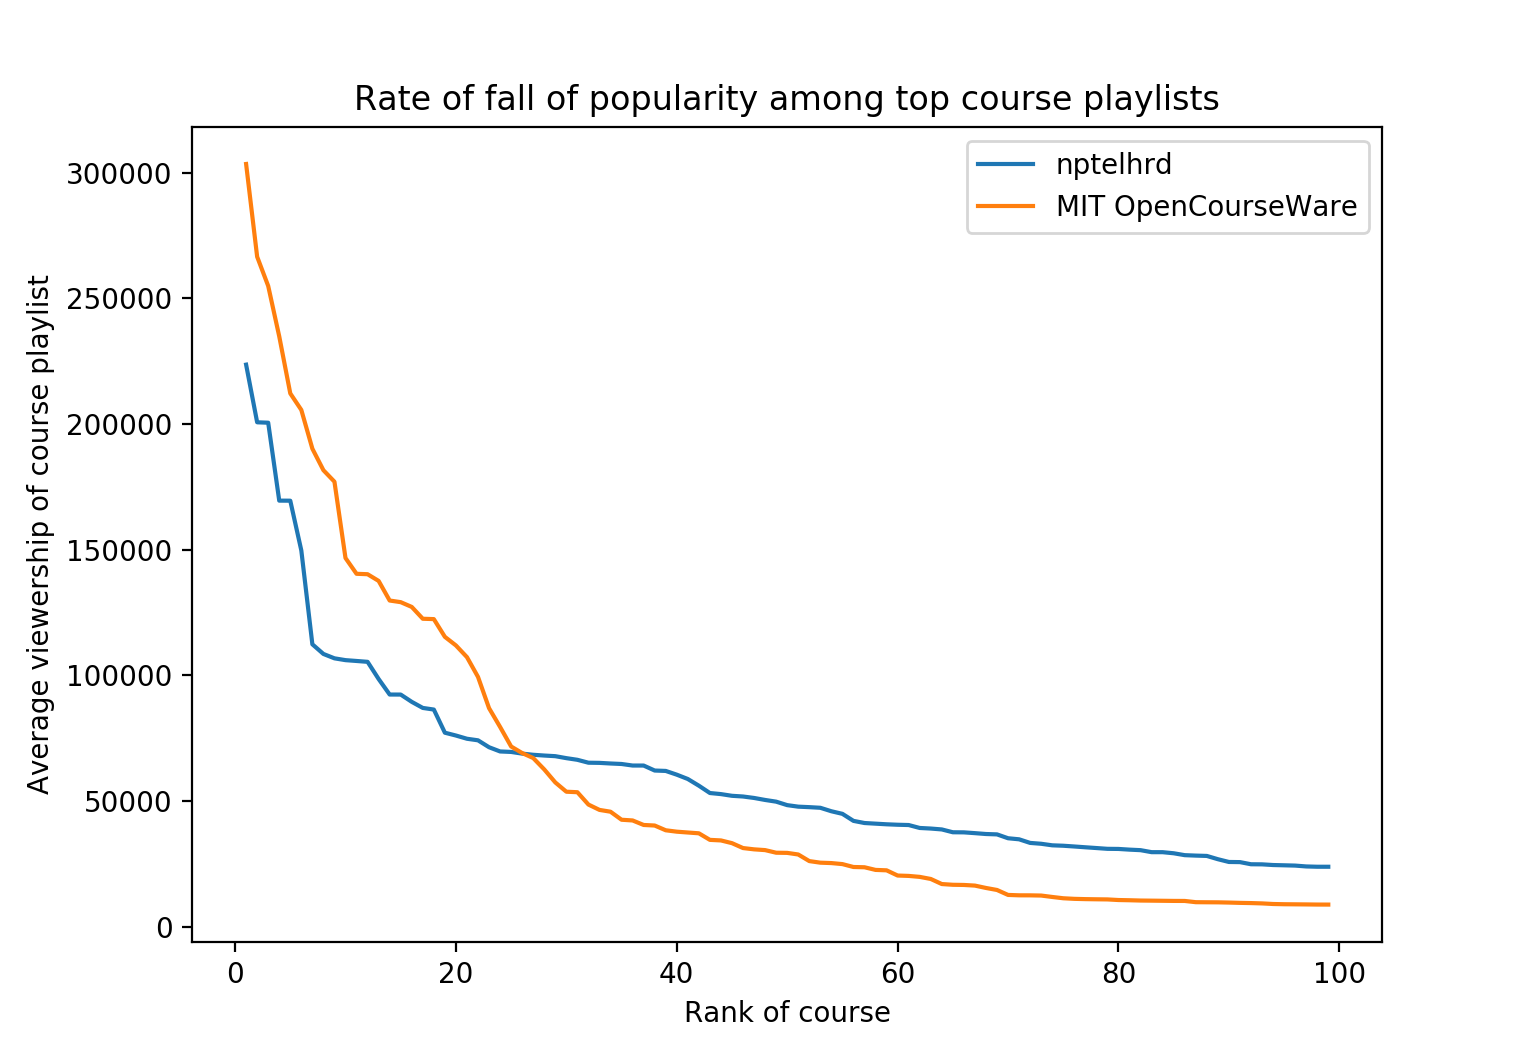
\includegraphics[scale=0.5]{images/fall_of_views.png}
    \caption{Comparison of fall of popularity among top topics}
    \label{fig:my_label}
\end{figure}
\FloatBarrier

Several important inferences can be drawn from the above tables, graphs and barplots:

\begin{itemize}
    \item Among the top 10 topics for NPTEL, the vast majority of views ($\sim$62.5\%) comes from only the first 3-5 topics, while for MITOCW this percentage is 58.6\%.\\
    \item We also observe that the fall of popularity among the top 10 topics is steeper for MITOCW than for NPTEL. In other words, only the first few topics of MITOCW are very popular.\\
    \item We see a difference of focus/perspective for both the channels. While NPTEL's popular courses are dominated by Computer Science, Mechanical and Electrical, covering all major domains of Engineering, MITOCW's top courses mainly consist of Math and Computer Science courses.\\
    \item In the top 100 list of topics obtained for MITOCW, we found at least 5 different topics relating to Finance/Economics (\textbf{Topics in Mathematics w Applications in Finance}, \textbf{Finance Theory I}, \textbf{Principles of Microeconomics}, \textbf{Development Economics: Macroeconomics}, \textbf{Poker Theory and Analysis}) while for NPTEL, there were almost none. We can conclusively say that NPTEL should publish more playlists focused towards the Economics and Financial domain.\\
\end{itemize}

We also created a mapping of similar/common topics among playlists of both the channels. This is tabularised below.

\begin{table}[!htpb]
    \centering
    \begin{tabular}{|c|c|c|c|}
        \hline
        \textbf{Rank} & \textbf{NPTEL Playlist Topic} & \textbf{Rank} & \textbf{MITOCW Playlist Topic}\\
        \hline
         5 & Data Structures and Algorithms & 13 & Introduction to Algorithms\\
         79 & Linear Algebra & 2 & Linear Algebra\\
         32 & Artifical Intelligence & 7 & Artificial Intelligence\\
         4 & Basic Electrical Circuits & 18 & Circuits and Electronics\\
         6 & Thermodynamics & 23 & Thermodynamics and Kinetics\\
         14 & Quantum Physics & 6 & Quantum Physics III\\
         17 & Advanced Digital Signal Processing & 42 & Digital Signal Processing\\
         \hline
    \end{tabular}\vspace{3mm}
    \caption{Mapping of similar topics from NPTEL and MITOCW}
    \label{tab:my_label}
\end{table}
\FloatBarrier

\noindent We find a couple of outliers in the mapping of topics shown above. In particular, Linear Algebra, being the basic foundation stone of various fields in Mathematics, Physics, and Computer Science, is highly popular in MITOCW's playlist. But the same course by NPTEL hasn't observed enough popularity. The same goes for the Artificial Intelligence course. It hence can be suggested that the existing playlists on NPTEL for Linear Algebra and Artificial Intelligence should be revised to better match the requirements of the current generation of research and development.\\


\subsection{Analysis of peaks of views in a playlist}
We did peak analysis on playlists using views gained by each video. We used anomaly detection for the task. Using the z-score as the metric, we look at the values where the curve diverges from that video's predicted values in the playlist. Below are a few graphs that we obtained. 

\begin{figure}[!htpb]
    \centering
    \subfloat[\centering Famous lecturers ]{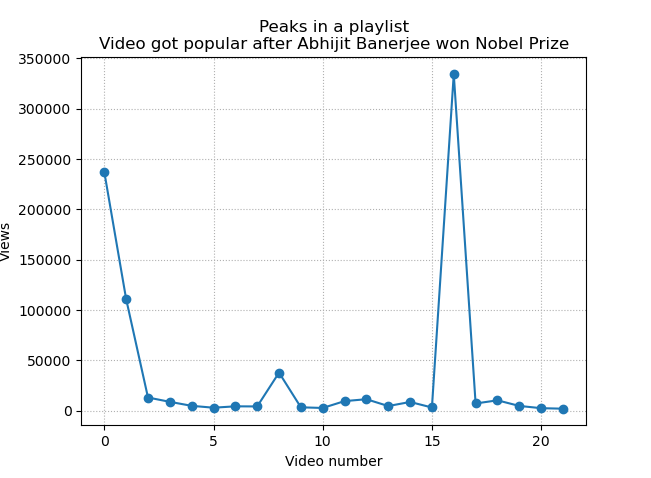
\includegraphics[width=0.51\textwidth ,height=5.5cm]{images/peak_graph2.png} \label{fig:img1}} \hspace{-3.5em}%
    \qquad
    \subfloat[\centering Interesting Title ]{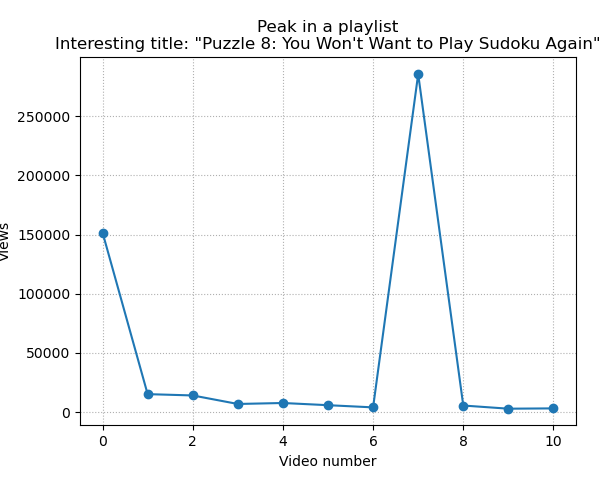
\includegraphics[width=0.51\textwidth,height=5.5cm]{images/peak_graph3.png} \label{fig:img2}
    }\\%
    \caption{Peak Analysis graphs - 1}
\end{figure}
\begin{figure}[!htpb]
    \centering
    \subfloat[Popular course topic: AJM]{\label{fig:a}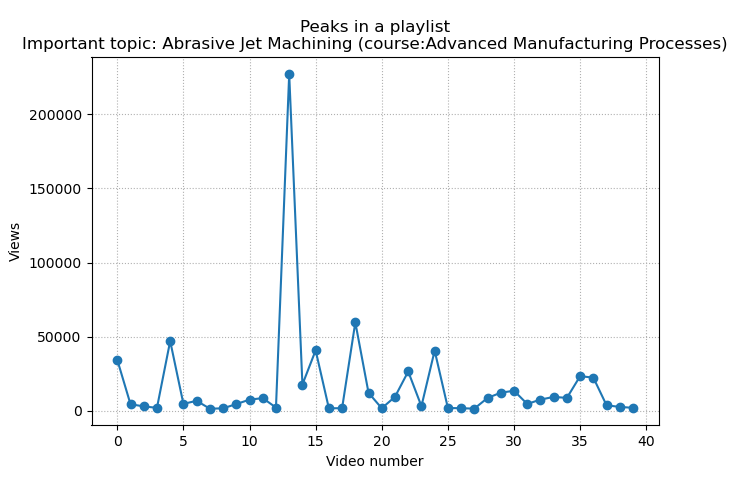
\includegraphics[width=0.50\textwidth,height=5.5cm]{images/peak_graph1.png} \label{fig:img3}} \hspace{-2.5em}%
    \qquad
    \subfloat[Popular course topic: Mechanical Vibration]{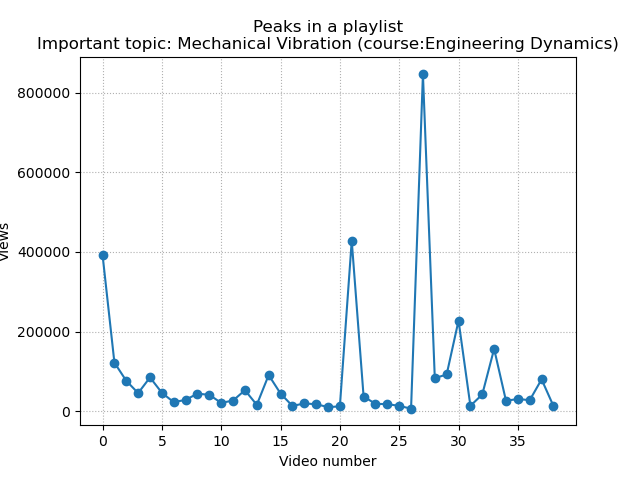
\includegraphics[width=0.50\textwidth,height=5.5cm]{images/peak_graph4.png} \label{fig:img4}}\\%
    \caption{Peak analysis graphs - 2}
\end{figure}
\FloatBarrier


After observing peaks on playlists, we closely looked at the playlist content and peak video content to investigate the reason behind the peaks. Below are a few interesting insights that we obtained about the peak videos in the playlist.
\begin{itemize}
    \item \textbf{Famous Guest lecturers:} We observed a sharp increase in view count for videos featuring special lecturers or famous guests. For an Aerospace course playlist on the MIT OCW channel, a sharp peak is observed for the video featuring \textbf{Lt Col Randy ``Laz'' Gordon} as a guest lecturer. Another instance is a lecture by \textbf{Abhijit Banerjee} \textbf{(see figure \ref{fig:img1}).} 
    \item \textbf{Important and Difficult to understand topics:}
    In our analysis, we observed that a sharp peak came for videos having obtrusive content. Such videos might need multiplied re-watches and thus contributes to the peak that we observed.
    For example, \textbf{Mechanical Vibration} (course: Engineering Dynamics) and \textbf{Abrasive Jet Machining} (course: Advanced manufacturing processes) are important and challenging topics for which students refer online resources \textbf{(see figure \ref{fig:img3} and \ref{fig:img4}).}  Not only do these peaks contribute to interesting findings from course data, but they also serve as insights to the instructors helping them focus more on topics that are tough to grasp by the students
    \item \textbf{Interesting titles:} We also found some peaks occurring because of interesting or tempting video titles. One such video titled "\textit{Puzzle 8: You Won't Want to Play Sudoku Again}" attracts the viewer and hence generate more views, compared to other videos on the playlists \textbf{(see figure \ref{fig:img2}).} Thus, including some videos with such titles might contribute to greater popularity of course playlists.
    \item \textbf{Common topics:} Videos on familiar topics and refresher videos in courses also gain large viewership compared to other videos. As these videos are fundamental in nature, they can cater to a wider variety of expertise and backgrounds. They are also some of the most used reference videos and thus attract more views than other videos of the course.  \textbf{(For example, Probability refreshers in the middle of a course)}
\end{itemize}


\subsection{Classifying Comments based on sentiment polarity}


The following table provides a few examples for assigning polarity to each comment - 

\begin{table}[!htbp]
\begin{adjustbox}{width=\columnwidth,center}
\begin{tabular}{|l|c|}
\hline
\multicolumn{1}{|c|}{\textbf{Comment Text}}                                                               & \textbf{Polarity Assigned} \\ \hline
The best part of NPTEL is we will be certified from one best Institute (IITs). Very Informative. & 0.73              \\ \hline
Is NPTEL courses only for engineering students \& engineering faculties?                         & 0                 \\ \hline
the voice breaks. annoying                                                                       & -0.8              \\ \hline
\end{tabular}\vspace{3mm}
\end{adjustbox}
\end{table}

 
Looking at the data, we found that the neutral comments talked more about the course logistics rather than the content. On the other hand, positive and negative comments expressed more about the course content.
 

What we found was the neutral comments were much more extensive in number than the negative comments. This observation tells us that more people were concerned about the course logistics (video quality, availability of slides, etc.)  rather than the video's content. It further motivates spending more on increasing video quality rather than spending on creating better content.
  
\begin{figure}[!htpb]
    \centering
    
    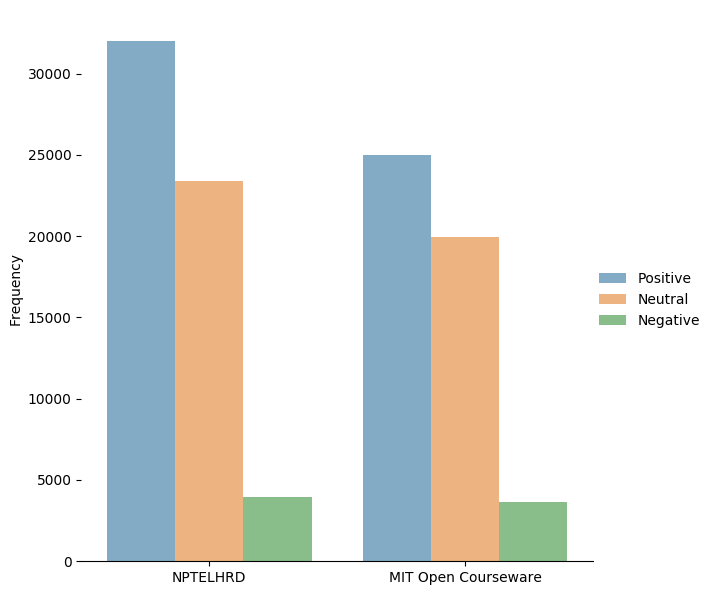
\includegraphics[width=8cm]{images/polarity_counts.png}%
    \caption{Frequency of Positive, Neutral and Negative comments}
    % \caption{Box plot of view and video length}%
    \label{fig:example}%
\end{figure}

\section{Conclusion}
The analysis of variation of the number of likes/views/comments with video length tells us that very short educational videos are not favored much by the users. Also, while longer videos can still get a substantial number of clicks on them, to have a high number of likes and comments, it is imperative to keep the video length around the mark of 10-15 minutes.

After comparing different IITs, IIT-D videos tend to be more popular, whereas IIT-KGP has published many videos across various topics. IIT Kanpur videos have good ratings, especially ones by CSE and EE departments.

Almost 80\% students who reach till $3^{rd}$ video in a course drop till they reach the $20^{th}$ video. The overall retention of higher-education channels (NPTEL, MIT) is much lower than that of high-school channels. This can be attributed to better quality videos and higher seriousness of students preparing for JEE. Also, retention of NPTEL is better than MIT, possibly due to the certification involved.

Popular courses in NPTEL span across more branches of engineering (CSE, EE, ME, CHE etc.), whereas those of MIT consist mostly of Maths and Computer Science. However, MIT has popular courses in non-engineering fields like Economics and Finance. Courses on Linear Algebra and Artificial Intelligence are highly popular on MIT but not on NPTEL, suggesting that IITs must revise these courses on NPTEL.

Anomalies in playlists can be used to find topics for which students are referring to online resources. These topics are important but challenging to grasp, and course instructors must teach them with more attention. For example, Abrasive Jet Machining from course Advanced manufacturing processes.

In the comments section, more people are concerned about the course logistics rather than course content. This indicates that NPTEL should focus on teaching and video quality rather than improving the contents of the course.

% The analysis has put forward some interesting insights. We found video length of around 10 min is optimal for maximum engagement with the audience. Strong coorelation exists between likes, views and comments. QS rankings are more closely related to popularity rather than quality of content. 


\section{Future Directions}
The Youtube Analytics API offers detailed information about videos which is only available to the owners of channel uploading the videos (NPTEL, MIT OCW etc. in this case). Aside from the analysis simply based on the number of views, we can use the Analytics API to see how individual sections of the videos are being watched, the average duration being watched, how many people are re-watching the videos, etc gain more insight into the topics. We can also use the demographics and location information of viewers to get interesting results.

We can also compare education videos with other categories (gaming, music, entertainment) to get interesting comparisons and parallels. This comparison might give us insights on how to increase quality and boost the popularity of educational videos.
\nocite{*}
\bibliographystyle{acm}
\bibliography{ref}

\end{document}